\documentclass{book}

\usepackage{cprog}
\usepackage{cc_manual}
\usepackage{cc_manual_index}
\usepackage{makeidx}
\usepackage{latex_converter}
\usepackage{amssymb}
\usepackage{graphicx}
\usepackage{path}
\usepackage{ipe}
\usepackage{alltt}
\usepackage{pslatex}
\usepackage{rotating}
\usepackage{psfrag}
\usepackage{minitoc}

% page dimensions
% ---------------
\textwidth 15.6cm 
\textheight 23 cm
\topmargin -14mm       
\evensidemargin 3mm 
\oddsidemargin 3mm

% default column layout
% ---------------------
\newcommand{\cgalColumnLayout}{\ccTexHtml{%
    \ccSetThreeColumns{CGAL_Oriented_side}{}{\hspace*{8.5cm}}
    \ccPropagateThreeToTwoColumns}{}}

\newcommand{\cgalrelease}{2.2-I-2}

\renewcommand{\ccRefPageBegin}{\ccParDims\cgalColumnLayout}
\ccDefGlobalScope{CGAL::}

% New manual style including tab markers on the side margins
% ----------------------------------------------------------
\marginparsep10mm
\marginparwidth15mm
\gdef\ccNewRefManualStyle{\ccFalse}  % undef this for old style manual

% The tab marker are aligned with the top of the main text. To align
% them with the page header, the following definition of the amount
% by which the tab is shifted can be used
\setlength{\ccRefTabLift}{12.5mm}

% Optionally, package authors and a package release can be shown
% right below the chapter title. Comment out the following lines
% to get back to the default behavior.
% -----------------------------------------------------------------
\def\ccTagChapterAuthor{\ccTrue}
\def\ccTagChapterRelease{\ccTrue}

\def\ccRefPageBegin{\ccParDims\cgalColumnLayout}
\def\ccRefPageEnd{\ccParDims\cgalColumnLayout}



\makeindex

\sloppy

%\ccTexHtml{\batchmode}{}

\begin{document}
\dominitoc
\tableofcontents

\pagenumbering{arabic}
 
% =============================================================================
% The CGAL Reference Manual
% Chapter: Optimisation
% -----------------------------------------------------------------------------
% file  : doc_tex/basic/Optimisation/main.tex
% author: Bernd G�rtner, Sven Sch�nherr (sven@inf.fu-berlin.de)
% -----------------------------------------------------------------------------
% $Revision$
% $Date$
% =============================================================================

\newcommand{\linebreakByHand}{\ccTexHtml{\\}{}}
\newcommand{\SaveSpaceByHand}{}  %%%% [2]{\ccTexHtml{#1}{#2}}

\chapter{Geometric Optimisation} \label{Optimisation}
\RCSdefDate{\OptRCSDate}{$Date$}

\ccChapterRelease{Release: 2.0 \ccTexHtml{\quad}{ , } \OptRCSDate}

\ccChapterAuthor{Bernd G{\"a}rtner}\ccTexHtml{\\}{<br>}
\ccChapterAuthor{Michael Hoffmann}\ccTexHtml{\\}{<br>}
\ccChapterAuthor{Sven Sch{\"o}nherr}

\ccTexHtml{\thispagestyle{empty}}{}

\begin{ccTexOnly}\section*{Introduction}\end{ccTexOnly}
\begin{ccHtmlOnly}<H2>Introduction</H2><P>\end{ccHtmlOnly}

This chapter describes routines for solving geometric optimisation problems.
The first two sections contain algorithms for computing and updating the
smallest enclosing circle (Section~\ref{sec:smallest_enclosing_circles})
resp.\ ellipse (Section~\ref{sec:smallest_enclosing_ellipses}) of a finite
point set.  Formally, the `smallest enclosing circle' is the boundary of the
closed disk of minimum area covering the point set. It is known that this
disk is unique.  We usually identify the disk with its bounding circle,
allowing us to talk about points being on the boundary of the circle, etc.
The same holds for the smallest enclosing ellipse. These algorithms work in
an incremental manner. They are implemented as semi-dynamic data structures,
thus allowing to insert points while maintaining the smallest enclosing
circle resp.\ ellipse.

The remaining sections describe algorithms for searching in matrices with
specific properties and some applications. In particular, there are
general implementations of
\begin{itemize}
  \item monotone matrix search (see Section~\ref{secMonotoneMatrixSearch}),
    which can be applied to compute
    \begin{itemize}
      \item extremal polygons of a convex polygon
        (see Section~\ref{secComputingExtremalPolygons}) \textit{or}
      \item all furthest neighbors for the vertices of a convex polygon
        (see Section~\ref{secAllFurthestNeighbors}),
    \end{itemize}
  \item and sorted matrix search (see Section~\ref{secSortedMatrixSearch}),
    which can be used to compute the $p$-centers of a planar point set
    (see Section~\ref{sec_RectangularPCenters}).
\end{itemize}

\subsubsection*{Traits Class}
The class and function templates are parameterized with a traits class
which defines the abstract interface between the optimisation
algorithm and the primitives it uses. We provide traits class
implementations that interface the optimisation algorithms with the
\cgal\ kernel. For some algorithms, in addition, we provide traits
class adapters to user supplied point classes. Finally, we describe
the requirements that must be fulfilled by traits classes for
optimisation algorithms.  This is at the same time a specification for
using the provided traits class implementations as for users who want
to supply their own traits class.

\subsubsection*{Assertions}
The optimisation code uses infix \ccc{OPTIMISATION} in the assertions,
e.g.\ defining the compiler flag
\ccc{CGAL_OPTIMISATION_NO_PRECONDITIONS} switches precondition
checking off, cf.~Section~\ref{assertions}.

\newcommand{\cgalSetOptTraitsAdaptLayout}{\ccTexHtml{%
    \ccSetThreeColumns{CGAL_Oriented_side}{}{returns constants
      \ccc{CGAL_LEFTTURN}, \ccc{CGAL_COLLINEAR}}
    \ccPropagateThreeToTwoColumns}{}}
\newcommand{\cgalSetOptTraitsAdaptReqLayout}{\ccTexHtml{%
    \ccSetThreeColumns{CGAL_Oriented_side}{da.get_hw( Point p).}{}
    \ccPropagateThreeToTwoColumns}{}}

\newcommand{\cgalSetOptTraitsReqLayout}{\ccTexHtml{%
    \ccSetThreeColumns{CGAL_Oriented_side}{}{returns
      \ccc{CGAL_ON_BOUNDED_SIDE}, \ccc{CGAL_ON_BOUNDARY}}
    \ccPropagateThreeToTwoColumns}{}}

\ccHtmlNoClassToc

\input{smallest_enclosing_circles}

\input{smallest_enclosing_ellipses}

%% ==============================================================
%% Specification: Computing Extremal Polygons
%% --------------------------------------------------------------
%% file  : spec_extremal_polygons.awi
%% author: Michael Hoffmann
%% $Id$
%% ==============================================================

\clearpage
\section{Computing Extremal Polygons}
\label{secComputingExtremalPolygons}
\cgalColumnLayout

This section describes several functions to compute a maximal $k$-gon
$P_k$ that can be inscribed into a given convex polygon $P$. The
criterion for maximality can be chosen freely by defining an
appropriate traits class as specified in section
\ref{req_ExtremalPolygonTraits}. For \cgal\ point classes there are
two predefined traits classes to compute a maximum area (see section
\ref{secMaximumAreaInscribedKgon}) resp.  perimeter (see section
\ref{secMaximumPerimeterInscribedKgon}) inscribed $k$-gon.

\ccHtmlNoClassToc
\begin{ccHtmlClassFile}{computing_maximum_area_inscribed_k_gon.html}
  {Function Declaration of \ccc{maximum_area_inscribed_k_gon}}
  \ccHtmlNoClassIndex\ccHtmlNoClassLinks
  %% class wrapper to keep the font at a uniform size:
  \begin{ccClass}{dummy}
    \ccHtmlNoIndex\subsection{Computing a Maximum Area Inscribed $k$-gon}
  \label{secMaximumAreaInscribedKgon}
  \end{ccClass}
  
  This section describes a function to compute a maximal area $k$-gon
  $P_k$ that can be inscribed into a given convex polygon $P$. Note
  that $P_k$ is not unique in general, but it can be chosen in such a
  way that its vertices form a subset of the vertex set of $P$.

  \ccInclude{CGAL/extremal_polygon_2.h}

  \def\ccLongParamLayout{\ccTrue} 
  
  \ccGlobalFunction{
    template < class RandomAccessIC, class OutputIterator >
    OutputIterator
    maximum_area_inscribed_k_gon(
    RandomAccessIC points_begin,
    RandomAccessIC points_end,
    int k,
    OutputIterator o);}
  
  computes a maximum area inscribed $k$-gon of the convex polygon
  described by [\ccc{points_begin}, \ccc{points_end}), writes its
  vertices to \ccc{o} and returns the past-the-end iterator of this
  sequence.
  
  \ccHeading{Precondition}
  \begin{enumerate}
  \item Value type of \ccc{RandomAccessIC} has to be
    \ccc{Point_2<R>} for some representation class \ccc{R}.
  \item \ccc{OutputIterator} accepts the value type of
    \ccc{RandomAccessIC} as value type,
  \item the -- at least three -- points denoted by the range
    [\ccc{points_begin}, \ccc{points_end}) form the boundary of a convex
    polygon (oriented clock-- or counterclockwise) \textit{and}
  \item $k \ge 3$.
  \end{enumerate}

  \ccHeading{Note}
  
  On compilers not supporting member function templates, the parameter
  \ccc{RandomAccessIC} is fixed to \ccc{vector<Point_2>::iterator}
  where \ccc{Point_2} is the value type of \ccc{RandomAccessIC}.
  
  \ccImplementation The implementation uses monotone matrix
  search\cite{akmsw-gamsa-87} and has a worst case running time of $O(k
  \cdot n + n \cdot \log n)$, where $n$ is the number of vertices in
  $P$.

  \ccExample The following code generates a random convex polygon
  \ccc{p} with ten vertices and computes the maximum area inscribed
  five-gon of \ccc{p}.

  \ccIncludeVerbatim{extremal_polygon_2_example_area.C}

\end{ccHtmlClassFile}
    
\ccHtmlNoClassToc
\begin{ccHtmlClassFile}{computing_maximum_perimeter_inscribed_k_gon.html}
  {Function Declaration of \ccc{maximum_perimeter_inscribed_k_gon}}
  \ccHtmlNoClassIndex\ccHtmlNoClassLinks
  %% class wrapper to keep the font at a uniform size:
  \begin{ccClass}{dummy}
    \ccHtmlNoIndex\subsection{Computing a Maximum Perimeter Inscribed
      $k$-gon}
    \label{secMaximumPerimeterInscribedKgon}
  \end{ccClass}
  
  This section describes a function to compute a largest perimeter
  $k$-gon $P_k$ that can be inscribed in a given convex polygon $P$.
  Note that $P_k$ is not unique in general, but we know that its
  vertices form a subset of the vertex set of $P$.

  \ccInclude{CGAL/extremal_polygon_2.h}

  \def\ccLongParamLayout{\ccTrue}
  \ccGlobalFunction{
    template < class RandomAccessIC, class OutputIterator >
    OutputIterator
    maximum_perimeter_inscribed_k_gon(
    RandomAccessIC points_begin,
    RandomAccessIC points_end,
    int k,
    OutputIterator o);}
  
  computes a maximum perimeter inscribed $k$-gon of the convex polygon
  described by [\ccc{points_begin}, \ccc{points_end}), writes its
  vertices to \ccc{o} and returns the past-the-end iterator of this
  sequence.

  \ccHeading{Precondition}
  \begin{enumerate}
  \item Value type of \ccc{RandomAccessIC} has to be
    \ccc{Point_2<R>} for some representation class \ccc{R},
  \item there is a global function \ccc{R::FT sqrt( R::FT)}
    defined that computes the squareroot of a number,
  \item \ccc{OutputIterator} accepts the value type of
    \ccc{RandomAccessIC} as value type,
  \item the -- at least three -- points denoted by the range
    [\ccc{points_begin}, \ccc{points_end}) form the boundary of a
    convex polygon (oriented clock-- or counterclockwise) \textit{and}
  \item $k \ge 2$.
  \end{enumerate}

  \ccTagDefaults

  \ccHeading{Note}
  
  On compilers not supporting member function templates, the parameter
  \ccc{RandomAccessIC} is fixed to \ccc{vector<Point_2>::iterator}
  where \ccc{Point_2} is the value type of \ccc{RandomAccessIC}.
  
  \ccImplementation The implementation uses monotone matrix
  search\cite{akmsw-gamsa-87} and has a worst case running time of $O(k
  \cdot n + n \cdot \log n)$, where $n$ is the number of vertices in
  $P$.

  \ccExample The following code generates a random convex polygon
  \ccc{p} with ten vertices and computes the maximum perimeter inscribed
  five-gon of \ccc{p}.

  \ccIncludeVerbatim{extremal_polygon_2_example_perimeter.C}

\end{ccHtmlClassFile}

\begin{ccAdvanced}
  \ccHtmlNoClassToc
  \begin{ccHtmlClassFile}{computing_general_extremal_polygons.html}
    {Function Declaration of \ccc{extremal_polygon}}
    \ccHtmlNoClassIndex\ccHtmlNoClassLinks
    %% class wrapper to keep the font at a uniform size:
    \begin{ccClass}{dummy}
      \ccHtmlNoIndex\subsection{Computing General Extremal
        Polygons}\label{secGeneralExtremalPolygons}
    \end{ccClass}
    
    This section describes a general function to compute a maximal
    $k$-gon $P_k$ that can be inscribed in a given convex polygon $P$.
    The criterion for maximality and some basic operations have to
    specified in an appropriate traits class as specified in section
    \ref{req_ExtremalPolygonTraits}.
    
    \ccInclude{CGAL/extremal_polygons_2.h}

    \def\ccLongParamLayout{\ccTrue} 
    
    \ccGlobalFunction{
      template < class RandomAccessIC, class OutputIterator, class Traits >
      OutputIterator
      extremal_polygon(
      RandomAccessIC points_begin,
      RandomAccessIC points_end,
      int k,
      OutputIterator o,
      const Traits& t);}
    
    computes a maximal (as specified by \ccc{t}) inscribed $k$-gon of
    the convex polygon described by [\ccc{points_begin},
    \ccc{points_end}), writes its vertices to \ccc{o} and returns the
    past-the-end iterator of this sequence.
    
    \ccHeading{Precondition}
    \begin{enumerate}
    \item \ccc{Traits} has to satisfy the requirements stated in section
      \ref{req_ExtremalPolygonTraits},
    \item Value type of \ccc{RandomAccessIC} must be
      \ccc{Traits::Point_2},
    \item \ccc{OutputIterator} accepts \ccc{Traits::Point_2} as value
      type,
    \item the -- at least three -- points denoted by the range
      [\ccc{points_begin}, \ccc{points_end}) form the boundary of a
      convex polygon (oriented clock-- or counterclockwise) \textit{and}
    \item $k \ge \ccc{t.min_k()}$.
    \end{enumerate}
    
    \ccImplementation The implementation uses monotone matrix
    search\cite{akmsw-gamsa-87} and has a worst case running time of
    $O(k \cdot n + n \cdot \log n)$, where $n$ is the number of vertices
    in $P$.
  \end{ccHtmlClassFile}
  
  \ccHtmlNoClassToc\ccHtmlNoClassIndex\begin{ccClass}{Exp_traits}
    \ccCreationVariable{t}\ccTagFullDeclarations
    
    \subsection{Requirements for Extremal Polygon Traits
      Classes}\label{req_ExtremalPolygonTraits}
    
    \ccDefinition A class \ccClassName\ has to provide the following
    types and operations in order to qualify as a traits class for
    \ccc{extremal_polygon}.
    
    \ccTypes 
    
    \ccNestedType{Point_2}{class used for representing the input
      points.}
    
    \ccNestedType{FT}{class used for doing computations on point
      coordinates (has to fulfill field-type requirements).}
    
    \ccNestedType{Operation}{AdaptableBinaryFunction class \ccc{op}:
      \ccc{Point_2} $\times$ \ccc{Point_2} $\rightarrow$ \ccc{FT}.
      Together with \ccc{init} this operation recursively defines the
      objective function to maximize.  Let $p$ and $q$ be two vertices
      of a polygon $P$ such that $q$ precedes $p$ in the oriented
      vertex chain of $P$ starting with vertex $root$.  Then
      \ccc{op(p,q)} returns the value by which an arbitrary
      sub-polygon of $P$ with vertices from $[root,\, q]$ increases
      when $p$ is added to it. E.g. in the maximum area case this is
      the area of the triangle $(root,\, q,\, p)$.}

    \ccOperations
    
    \ccMemberFunction{int min_k() const;}{returns the minimal $k$ for
      which a maximal $k$-gon can be computed. (e.g. in the maximum
      area case this is three.)}
    
    \ccMemberFunction{FT init( const Point_2& p, const Point_2& q)
      const;}{returns the value of the objective function for a
      polygon consisting of the two points \ccc{p} and \ccc{q}. (e.g.
      in the maximum area case this is \ccc{FT( 0)}.)}
    
    \ccMemberFunction{Operation operation( const Point_2& p)
      const;}{return \ccc{Operation} where \ccc{p} is the fixed $root$
      point.}
    
    \ccMemberFunction{template < class RandomAccessIC, class
      OutputIterator > OutputIterator compute_min_k_gon(
      RandomAccessIC points_begin, RandomAccessIC points_end, FT&
      max_area, OutputIterator o) const;}{writes the points of
      [\ccc{points_begin}, \ccc{points_end}) forming a
      \ccc{min_k()}-gon rooted at \ccc{points_begin[0]} of maximal
      value to o and returns the past-the-end iterator for that
      sequence (== \ccc{o + min_k()}).}
    
    \ccMemberFunction{template < class RandomAccessIC > bool
      is_convex( RandomAccessIC points_begin, RandomAccessIC
      points_end) const;}{returns true, iff the points
      [\ccc{points_begin}, \ccc{points_end}) form a convex chain.}
    
    \ccHeading{Notes}
    \begin{itemize}
    \item \ccClassName\ccc{::is_convex} is only used for precondition
      checking. Therefore it needs not to be specified, in case that
      precondition checking is disabled.
    \item On compilers not supporting member function templates,
      \ccc{RandomAccessIC} is fixed to \ccc{vector<Point_2>::iterator}
      and \ccc{OutputIterator} is fixed to
      \ccc{vector<int>::reverse_iterator}.
      
    \end{itemize}
    
    \ccSeeAlso \ccInclude{CGAL/Extremal_polygon_traits_2.h}
    
    The classes \ccc{Kgon_area_traits<R>} and
    \ccc{Kgon_perimeter_traits<R>} (templatized with a \cgal\ 
    representation class) both fulfill these requirements.
    
  \end{ccClass}
\end{ccAdvanced}

%% --------------------------------------------------------------
%% EOF spec_extremal_polygons.awi
%% --------------------------------------------------------------

 
%% ==============================================================
%% Specification: All Furthest Neighbors
%% --------------------------------------------------------------
%% file  : spec_all_furthest_neighbors.awi
%% author: Michael Hoffmann
%% $Id$
%% ==============================================================

\cgalColumnLayout

\begin{ccRefFunction}{all_furthest_neighbors_2}
  
  \ccDefinition The function \ccRefName\ computes all furthest
  neighbors for the vertices of a convex polygon $P$, i.e. for each
  vertex $v$ of $P$ a vertex $f_v$ of $P$ such that the distance
  between $v$ and $f_v$ is maximized.

  \ccInclude{CGAL/all_furthest_neighbors_2.h}

  \def\ccLongParamLayout{\ccTrue} 
  
  \ccGlobalFunction{ template < class RandomAccessIC, class
    OutputIterator, class Traits > OutputIterator
    all_furthest_neighbors_2( RandomAccessIC points_begin,
    RandomAccessIC points_end, OutputIterator o, Traits t =
    Default_traits);}
  
  computes all furthest neighbors for the vertices of the convex
  polygon described by the range [\ccc{points_begin},
  \ccc{points_end}), writes their indices (relative to
  \ccc{points_begin}) to \ccc{o}\footnote{i.e. the furthest neighbor
    of \ccc{points_begin[}i\ccc{]} is \ccc{points_begin[}$i$-th number
    written to \ccc{o}\ccc{]}} and returns the past-the-end iterator
  of this sequence.
  
  \ccPrecond The points denoted by the non-empty range
  [\ccc{points_begin}, \ccc{points_end}) form the boundary of a convex
  polygon $P$ (oriented clock-- or counterclockwise).
  
  The geometric types and operations to be used for the computation
  are specified by the traits class parameter \ccc{t}. This parameter
  can be omitted if \ccc{RandomAccessIC} refers to a point type from
  the 2D-Kernel. In this case, a default traits class
  (\ccc{All_furthest_neighbors_default_traits_2<R>}) is used.
  
  \ccRequire
  \begin{enumerate}
  \item If \ccc{t} is specified explicitly, \ccc{Traits} is a model
    for \ccc{All_furthest_neighbors_traits_2}.
  \item Value type of \ccc{RandomAccessIC} is \ccc{Traits::Point_2} or
    -- if \ccc{t} is not specified explicitly -- \ccc{Point_2<R>} for
    some representation class \ccc{R}.
  \item \ccc{OutputIterator} accepts \ccc{int} as value type.
  \end{enumerate}
  
  \ccSeeAlso
  \ccRefIdfierPage{All_furthest_neighbors_traits_2}\\
  \ccRefIdfierPage{CGAL::All_furthest_neighbors_default_traits_2<R>}\\
  \ccRefIdfierPage{CGAL::monotone_matrix_search}
 
  \ccImplementation The implementation uses monotone matrix
  search\cite{akmsw-gamsa-87}. Its runtime complexity is linear in the
  number of vertices of $P$.
  
  \ccExample The following code generates a random convex polygon
  \ccc{p} with ten vertices, computes all furthest neighbors and
  writes the sequence of their indices (relative to
  \ccc{points_begin}) to \ccc{cout} (e.g. a sequence of
  \ccc{4788911224} means the furthest neighbor of
  \ccc{points_begin[0]} is \ccc{points_begin[4]}, the furthest
  neighbor of \ccc{points_begin[1]} is \ccc{points_begin[7]} etc.).
  
  \ccIncludeVerbatim{Optimisation_ref/all_furthest_neighbors_2_example_noheader.C}
\end{ccRefFunction}

\begin{ccRefClass}{All_furthest_neighbors_default_traits_2<R>}
  \ccCreationVariable{t}\ccTagFullDeclarations
  
  \ccDefinition The class \ccClassName\ provides the types and
  operations needed to compute all furthest neighbors for the vertices
  of a convex polygon.
  
  \ccRequirements
  The template parameter \ccc{R} is a model for \ccc{Kernel}.

  \ccIsModel 
  \ccRefIdfierPage{All_furthest_neighbors_traits_2}

  \ccTypes
  
  \ccNestedType{Point_2}{typedef to \ccc{R::Point_2}.}
  
  \ccNestedType{FT}{typedef to \ccc{R::FT}.}
  
  \ccNestedType{Distance}{AdaptableBinaryFunction class: \ccc{Point_2}
    $\times$ \ccc{Point_2} $\rightarrow$ \ccc{FT} computing the
    squared Euclidean distance between two points.}

  \ccOperations
  
  \ccMemberFunction{Distance distance_object();}{returns the
    function object for computing distances.}
  
  \ccMemberFunction{template < class RandomAccessIC > bool is_convex(
    RandomAccessIC points_begin, RandomAccessIC points_end)
    const;}{returns true, iff the points [\ccc{points_begin},
    \ccc{points_end}) form a convex chain.}
  
  \ccSeeAlso
  \ccRefIdfierPage{CGAL::all_furthest_neighbors_2}

  \ccHeading{Notes}
  \begin{itemize}
  \item \ccClassName\ccc{::is_convex} is used for precondition
    checking only.
  \end{itemize}
\end{ccRefClass}

\begin{ccRefConcept}{All_furthest_neighbors_traits_2}
  \ccCreationVariable{t}\ccTagFullDeclarations
  
  \ccDefinition The concept \ccRefName\ defines types and operations
  needed to compute all furthest neighbors for the vertices of a
  convex polygon using the function \ccc{all_furthest_neighbors_2}.
  
  \ccTypes
  
  \ccNestedType{Point_2}{class used for representing the input
    points.}
  
  \ccNestedType{FT}{class used for doing computations on point
    coordinates; it has to be a model for \ccc{FieldNumberType}.}
  
  \ccNestedType{Distance}{AdaptableBinaryFunction class: \ccc{Point_2}
    $\times$ \ccc{Point_2} $\rightarrow$ \ccc{FT} computing the
    squared Euclidean distance between two points.}

  \ccOperations
  
  \ccMemberFunction{Distance distance_object();}{returns the
    function object for computing distances.}
  
  \ccMemberFunction{template < class RandomAccessIC > bool is_convex(
    RandomAccessIC points_begin, RandomAccessIC points_end)
    const;}{returns true, iff the points [\ccc{points_begin},
    \ccc{points_end}) form a convex chain.}
  
  \ccHasModels 
  \ccRefIdfierPage{CGAL::All_furthest_neighbors_default_traits_2<R>}

  \ccSeeAlso
  \ccRefIdfierPage{CGAL::all_furthest_neighbors_2}

  \ccHeading{Notes}
  \begin{itemize}
  \item \ccClassName\ccc{::is_convex} is used for precondition
    checking only.
  \end{itemize}
\end{ccRefConcept}

%% --------------------------------------------------------------
%% EOF spec_all_furthest_neighbors.awi
%% --------------------------------------------------------------

 
%% ==============================================================
%% Specification: Rectangular p-Centers
%% --------------------------------------------------------------
%% file  : spec_rectangular_p_centers.awi
%% author: Michael Hoffmann
%% $Id$
%% ==============================================================

\cgalColumnLayout

\begin{ccRefFunction}{rectangular_p_center_2}
  \ccIndexMainItem[t]{rectilinear centers}
  \ccIndexMainItem[t]{rectangular centers}
  \ccIndexSubitem[t]{center}{rectangular}
  
  \ccDefinition The function \ccRefName\ computes rectilinear
  $p$-centers of a planar point set, i.e. a set of $p$ points such
  that the maximum minimal $L_{\infty}$-distance between both sets is
  minimized.
  
  More formally the problem can be defined as follows.
  
  \ccTexHtml{Given a finite set $\mathcal{P}$ of points, compute a
    point set $\mathcal{C}$ with $|\mathcal{C}| \le p$ such that the
    $p$-radius of $\mathcal{P}$,
    $$
    rad_p(\mathcal{P}) := \max_{P \in \mathcal{P}} \min_{Q \in
      \mathcal{C}} || P - Q ||_\infty
    $$
    is minimized. We can interpret $\mathcal{C}$ as the best
    approximation (with respect to the given metric) for $\mathcal{P}$
    with at most $p$ points.}{Given a finite set <IMG WIDTH=12
    HEIGHT=12 ALIGN=BOTTOM ALT="tex2html_wrap_inline17"
    SRC="./MatrixSearch_pcenter1.gif" > of points, compute a point set
    <IMG WIDTH=9 HEIGHT=13 ALIGN=BOTTOM ALT="tex2html_wrap_inline19"
    SRC="./MatrixSearch_pcenter2.gif" > with <IMG WIDTH=46 HEIGHT=24
    ALIGN=MIDDLE ALT="tex2html_wrap_inline21"
    SRC="./MatrixSearch_pcenter3.gif" > such that the <I>p</I>-radius
    of <IMG WIDTH=12 HEIGHT=12 ALIGN=BOTTOM
    ALT="tex2html_wrap_inline17" SRC="./MatrixSearch_pcenter1.gif" > ,
    <P> <IMG WIDTH=358 HEIGHT=24 ALIGN=BOTTOM ALT="displaymath27"
    SRC="./MatrixSearch_pcenter4.gif" > <P> is minimized. We can
    interpret <IMG WIDTH=9 HEIGHT=13 ALIGN=BOTTOM
    ALT="tex2html_wrap_inline19" SRC="./MatrixSearch_pcenter2.gif" >
    as the best approximation (with respect to the given metric) for
    <IMG WIDTH=12 HEIGHT=12 ALIGN=BOTTOM ALT="tex2html_wrap_inline17"
    SRC="./MatrixSearch_pcenter1.gif" > with at most <I>p</I> points.}

  \ccInclude{CGAL/rectangular_p_center_2.h}

  \def\ccLongParamLayout{\ccTrue} 
  
  \ccGlobalFunction{template < class ForwardIterator, class
    OutputIterator, class FT, class Traits > OutputIterator
    rectangular_p_center_2(ForwardIterator f, ForwardIterator l,
    OutputIterator o, FT& r, int p, const Traits& t =
    Default_traits);}
  
  computes rectilinear \ccc{p}-centers for the point set described by
  the range [\ccc{f}, \ccc{l}), sets \ccc{r} to the corresponding
  $p$-radius, writes the at most \ccc{p} center points to \ccc{o} and
  returns the past-the-end iterator of this sequence.
  
  \ccPrecond
  \begin{enumerate}
  \item The range [\ccc{f}, \ccc{l}) is not empty.
  \item 2 $\le$ \ccc{p} $\le$ 4.
  \end{enumerate}
  
  The geometric types and operations to be used for the computation
  are specified by the traits class parameter \ccc{t}. This parameter
  can be omitted if \ccc{ForwardIterator} refers to a point type from
  the 2D-Kernel. In this case, a default traits class
  (\ccc{Rectangular_p_center_default_traits_2<R>}) is used.
  
  \ccRequire
  \begin{enumerate}
  \item \textit{Either: (if no traits parameter is given)} Value type
    of \ccc{ForwardIterator} is \ccc{CGAL::Point_2<R>} for some
    representation class \ccc{R} and \ccc{FT} is equivalent to
    \ccc{R::FT},
  \item \textit{Or: (if a traits parameter is specified)} \ccc{Traits}
    is a model for \ccc{RectangularPCenterTraits_2}.
  \item \ccc{OutputIterator} accepts the value type of
    \ccc{ForwardIterator} as value type.
  \end{enumerate}  
  
  \ccSeeAlso
  \ccRefConceptPage{RectangularPCenterTraits_2}\\
  \ccRefIdfierPage{CGAL::Rectangular_p_center_default_traits_2<R>}\\
  \ccRefIdfierPage{CGAL::sorted_matrix_search}
  
  \ccImplementation The runtime is linear for $p \in \{2,\,3\}$ and
  $\mathcal{O}(n \cdot \log n)$ for $p = 4$ where $n$ is the number of
  input points. These runtimes are worst case optimal. The $3$-center
  algorithm uses a prune-and-search technique described in
  \cite{cgal:h-slacr-99}.  The $4$-center implementation uses sorted matrix
  search \cite{fj-fkppc-83,fj-gsrsm-84} and fast algorithms for
  piercing rectangles \cite{sw-rpppp-96}.
  
  \ccExample The following code generates a random set of ten points
  and computes its two-centers.

  \ccIncludeExampleCode{Matrix_search/rectangular_p_center_2_example_nohead.cpp}
\end{ccRefFunction}

\begin{ccRefClass}{Rectangular_p_center_default_traits_2<R>}
  \ccCreationVariable{t}\ccTagFullDeclarations
    
  \ccDefinition The class \ccRefName\ defines types and operations
  needed to compute rectilinear $p$-centers of a planar point set
  using the function \ccc{rectangular_p_center_2}.
  
  \ccRequirements The template parameter \ccc{R} is a model for
  \ccc{Kernel}.
  
  \ccIsModel
  \ccRefConceptPage{RectangularPCenterTraits_2}

  \ccTypes 
    
  \ccNestedType{FT}{typedef to \ccc{R::FT}.}
  
  \ccNestedType{Point_2}{typedef to \ccc{R::Point_2}.}
  
  \ccNestedType{Iso_rectangle_2}{typedef to \ccc{R::Iso_rectangle_2}.}
  
  \ccNestedType{Less_x_2}{typedef to \ccc{R::Less_x_2}.}
 
  \ccNestedType{Less_y_2}{typedef to \ccc{R::Less_y_2}.}
  
  \ccNestedType{Construct_vertex_2}{typedef to
    \ccc{R::Construct_vertex_2}.}
  
  \ccNestedType{Construct_iso_rectangle_2}{typedef to
    \ccc{R::Construct_iso_rectangle_2}.}
    
  \ccNestedType{Signed_x_distance_2}{adaptable binary function
    class: \ccc{Point_2} $\times$ \ccc{Point_2} $\rightarrow$
    \ccc{FT} returns the signed distance of two points'
    $x$-coordinates.}
  
  \ccNestedType{Signed_y_distance_2}{adaptable binary function
    class: \ccc{Point_2} $\times$ \ccc{Point_2} $\rightarrow$
    \ccc{FT} returns the signed distance of two points'
    $y$-coordinates.}
  
  \ccNestedType{Infinity_distance_2}{adaptable binary function
    class: \ccc{Point_2} $\times$ \ccc{Point_2} $\rightarrow$
    \ccc{FT} returns the $||\cdot||_{\infty}$ distance of two
    points.}
  
  \ccNestedType{Signed_infinity_distance_2}{adaptable binary
    function class: \ccc{Point_2} $\times$ \ccc{Point_2}
    $\rightarrow$ \ccc{FT} returns the signed $||\cdot||_{\infty}$
    distance of two points.}
  
  \ccNestedType{Construct_point_2_below_left_implicit_point_2}{
    3-argument function class: \ccc{Point_2} $\times$ \ccc{Point_2}
    $\times$ \ccc{FT} $\rightarrow$ \ccc{Point_2}. For arguments
    $(p,\,q,\,r)$ it returns the lower-left corner of the iso-oriented
    square with sidelength $r$ and upper-right corner at the
    intersection of the vertical line through $p$ and the horizontal
    line through $q$.}
    
  \ccNestedType{Construct_point_2_below_right_implicit_point_2}{
    3-argument function class: \ccc{Point_2} $\times$ \ccc{Point_2}
    $\times$ \ccc{FT} $\rightarrow$ \ccc{Point_2}. For arguments
    $(p,\,q,\,r)$ it returns the lower-right corner of the
    iso-oriented square with sidelength $r$ and upper-left corner at
    the intersection of the vertical line through $p$ and the
    horizontal line through $q$.}
    
  \ccNestedType{Construct_point_2_above_right_implicit_point_2}{
    3-argument function class: \ccc{Point_2} $\times$ \ccc{Point_2}
    $\times$ \ccc{FT} $\rightarrow$ \ccc{Point_2}. For arguments
    $(p,\,q,\,r)$ it returns the upper-right corner of the
    iso-oriented square with sidelength $r$ and lower-left corner at
    the intersection of the vertical line through $p$ and the
    horizontal line through $q$.}
    
  \ccNestedType{Construct_point_2_above_left_implicit_point_2}{
    3-argument function class: \ccc{Point_2} $\times$ \ccc{Point_2}
    $\times$ \ccc{FT} $\rightarrow$ \ccc{Point_2}. For arguments
    $(p,\,q,\,r)$ it returns the upper-left corner of the iso-oriented
    square with sidelength $r$ and lower-right corner at the
    intersection of the vertical line through $p$ and the horizontal
    line through $q$.}

  \ccOperations
  
  For every function class listed above there is a member function
  to fetch the corresponding function object.
  
  \ccMemberFunction{Inf_distance_2 inf_distance_2_object() const;}{}
  \ccGlue\ccMemberFunction{Signed_inf_distance_2
    signed_inf_distance_2_object() const;}{}
  
  \ccGlue\ccMemberFunction{Construct_vertex_2
    construct_vertex_2_object() const;}{}
  
  \ccGlue\ccMemberFunction{Construct_iso_rectangle_2
    construct_iso_rectangle_2_object() const;}{}
  
  \ccGlue\ccMemberFunction{Construct_iso_rectangle_2_below_left_point_2
    construct_iso_rectangle_2_below_left_point_2_object() const;}{}
  
  \ccGlue\ccMemberFunction{Construct_iso_rectangle_2_above_left_point_2
    construct_iso_rectangle_2_above_left_point_2_object() const;}{}
  
  \ccGlue\ccMemberFunction{Construct_iso_rectangle_2_below_right_point_2
    construct_iso_rectangle_2_below_right_point_2_object() const;}{}
  
  \ccGlue\ccMemberFunction{Construct_iso_rectangle_2_above_right_point_2
    construct_iso_rectangle_2_above_right_point_2_object() const;}{}
  
  \ccSeeAlso
  \ccRefIdfierPage{CGAL::rectangular_p_center_2}

\end{ccRefClass}

\begin{ccRefConcept}{RectangularPCenterTraits_2}
  \ccCreationVariable{t}\ccTagFullDeclarations
    
  \ccDefinition The concept \ccRefName\ defines types and operations
  needed to compute rectilinear $p$-centers of a planar point set
  using the function \ccc{rectangular_p_center_2}.
  
  \ccTypes 
    
  \ccNestedType{FT}{model for \ccRefConceptPage{FieldNumberType}.}
  
  \ccNestedType{Point_2}{model for
    \ccRefConceptPage{Kernel::Point_2}.}
  
  \ccNestedType{Iso_rectangle_2}{model for
    \ccRefConceptPage{Kernel::Iso_rectangle_2}.}
  
  \ccNestedType{Less_x_2}{model for
    \ccRefConceptPage{Kernel::Less_x_2}.}
  
  \ccNestedType{Less_y_2}{model for
    \ccRefConceptPage{Kernel::Less_y_2}.}
  
  \ccNestedType{Construct_vertex_2}{model for
    \ccRefConceptPage{Kernel::Construct_vertex_2}.}
  
  \ccNestedType{Construct_iso_rectangle_2}{model for
    \ccRefConceptPage{Kernel::Construct_iso_rectangle_2}.}
    
  \ccNestedType{Signed_x_distance_2}{adaptable binary function
    class: \ccc{Point_2} $\times$ \ccc{Point_2} $\rightarrow$
    \ccc{FT} returns the signed distance of two points'
    $x$-coordinates.}
  
  \ccNestedType{Signed_y_distance_2}{adaptable binary function
    class: \ccc{Point_2} $\times$ \ccc{Point_2} $\rightarrow$
    \ccc{FT} returns the signed distance of two points'
    $y$-coordinates.}
  
  \ccNestedType{Infinity_distance_2}{adaptable binary function
    class: \ccc{Point_2} $\times$ \ccc{Point_2} $\rightarrow$
    \ccc{FT} returns the $||\cdot||_{\infty}$ distance of two
    points.}
  
  \ccNestedType{Signed_infinity_distance_2}{adaptable binary
    function class: \ccc{Point_2} $\times$ \ccc{Point_2}
    $\rightarrow$ \ccc{FT} returns the signed $||\cdot||_{\infty}$
    distance of two points.}
  
  \ccNestedType{Construct_point_2_below_left_implicit_point_2}{
    3-argument function class: \ccc{Point_2} $\times$ \ccc{Point_2}
    $\times$ \ccc{FT} $\rightarrow$ \ccc{Point_2}. For arguments
    $(p,\,q,\,r)$ it returns the lower-left corner of the iso-oriented
    square with sidelength $r$ and upper-right corner at the
    intersection of the vertical line through $p$ and the horizontal
    line through $q$.}
    
  \ccNestedType{Construct_point_2_below_right_implicit_point_2}{
    3-argument function class: \ccc{Point_2} $\times$ \ccc{Point_2}
    $\times$ \ccc{FT} $\rightarrow$ \ccc{Point_2}. For arguments
    $(p,\,q,\,r)$ it returns the lower-right corner of the
    iso-oriented square with sidelength $r$ and upper-left corner at
    the intersection of the vertical line through $p$ and the
    horizontal line through $q$.}
    
  \ccNestedType{Construct_point_2_above_right_implicit_point_2}{
    3-argument function class: \ccc{Point_2} $\times$ \ccc{Point_2}
    $\times$ \ccc{FT} $\rightarrow$ \ccc{Point_2}. For arguments
    $(p,\,q,\,r)$ it returns the upper-right corner of the
    iso-oriented square with sidelength $r$ and lower-left corner at
    the intersection of the vertical line through $p$ and the
    horizontal line through $q$.}
    
  \ccNestedType{Construct_point_2_above_left_implicit_point_2}{
    3-argument function class: \ccc{Point_2} $\times$ \ccc{Point_2}
    $\times$ \ccc{FT} $\rightarrow$ \ccc{Point_2}. For arguments
    $(p,\,q,\,r)$ it returns the upper-left corner of the iso-oriented
    square with sidelength $r$ and lower-right corner at the
    intersection of the vertical line through $p$ and the horizontal
    line through $q$.}

  \ccOperations
  
  For every function class listed above there is a member function
  to fetch the corresponding function object.
  
  \ccMemberFunction{Inf_distance_2 inf_distance_2_object() const;}{}
  \ccGlue\ccMemberFunction{Signed_inf_distance_2
    signed_inf_distance_2_object() const;}{}
  
  \ccGlue\ccMemberFunction{Construct_vertex_2
    construct_vertex_2_object() const;}{}
  
  \ccGlue\ccMemberFunction{Construct_iso_rectangle_2
    construct_iso_rectangle_2_object() const;}{}
  
  \ccGlue\ccMemberFunction{Construct_iso_rectangle_2_below_left_point_2
    construct_iso_rectangle_2_below_left_point_2_object() const;}{}
  
  \ccGlue\ccMemberFunction{Construct_iso_rectangle_2_above_left_point_2
    construct_iso_rectangle_2_above_left_point_2_object() const;}{}
  
  \ccGlue\ccMemberFunction{Construct_iso_rectangle_2_below_right_point_2
    construct_iso_rectangle_2_below_right_point_2_object() const;}{}
  
  \ccGlue\ccMemberFunction{Construct_iso_rectangle_2_above_right_point_2
    construct_iso_rectangle_2_above_right_point_2_object() const;}{}
  
  \ccHasModels
  \ccRefIdfierPage{CGAL::Rectangular_p_center_default_traits_2<R>}

  \ccSeeAlso
  \ccRefIdfierPage{CGAL::rectangular_p_center_2}

\end{ccRefConcept}

%% --------------------------------------------------------------
%% EOF spec_rectangular_p_centers.awi
%% --------------------------------------------------------------

 
%% ==============================================================
%% Specification: Monotone Matrix Search
%% --------------------------------------------------------------
%% file  : spec_monotone_matrix_search.awi
%% author: Michael Hoffmann
%% $Id$
%% ==============================================================

\cgalColumnLayout

\begin{ccRefFunction}{monotone_matrix_search}
  \begin{ccAdvanced}
    
    \ccDefinition The function \ccRefName\ computes the maxima for all
    rows of a totally monotone matrix.
    
    More precisely, monotony for matrices is defined as follows.
    
    \ccTexHtml{Let $K$ be a totally ordered set, $M \in K^{(n,\, m)}$
      a matrix over $K$ and for $0 \le i < n$:
      $$
      rmax_M(i) :\in \left\{ \min_{0 \le j < m} j \: \left|\:
          M[i,\, j] = \max_{0 \le k < m} M[i,\, k] \right.\right\}
      $$
      the (leftmost) column containing the maximum entry in row
      $i$.  $M$ is called monotone, iff
      $$
      \forall\, 0 \le i_1 < i_2 < n\: :\: rmax_M(i_1) \le
      rmax_M(i_2)\; .
      $$
      $M$ is totally monotone, iff all of its submatrices are
      monotone (or equivalently: iff all $2 \times 2$ submatrices are
      monotone).}{Let <I>K</I> be a totally ordered set, <IMG WIDTH=84
      HEIGHT=31 ALIGN=MIDDLE ALT="tex2html_wrap_inline11"
      SRC="./MatrixSearch_totmon1.gif" > a matrix over <I>K</I> and
      for <IMG WIDTH=64 HEIGHT=24 ALIGN=MIDDLE
      ALT="tex2html_wrap_inline13" SRC="./MatrixSearch_totmon2.gif" >
      : <P> <IMG WIDTH=427 HEIGHT=39 ALIGN=BOTTOM ALT="displaymath15"
      SRC="./MatrixSearch_totmon3.gif" > <P> the (leftmost) column
      containing the maximum entry in row <I>i</I>.  <I>M</I> is
      called monotone, iff <P> <IMG WIDTH=411 HEIGHT=16 ALIGN=BOTTOM
      ALT="displaymath19" SRC="./MatrixSearch_totmon4.gif" > <P>
      <I>M</I> is totally monotone, iff all of its submatrices are
      monotone (or equivalently: iff all <IMG WIDTH=33 HEIGHT=20
      ALIGN=MIDDLE ALT="tex2html_wrap_inline21"
      SRC="./MatrixSearch_totmon5.gif" > submatrices are monotone).}
    
    \ccInclude{CGAL/monotone_matrix_search.h}

    \def\ccLongParamLayout{\ccTrue} 
    \ccTexHtml{%
      \ccSetThreeColumns{void}{}{\hspace*{8.5cm}}
      \ccPropagateThreeToTwoColumns}{}
    
    \ccGlobalFunction{template < class Matrix, class RandomAccessIC,
      class Compare_strictly > void monotone_matrix_search( const
      Matrix& m, RandomAccessIC t, const Compare_strictly&
      compare_strictly = less< Matrix::Value >());}
    
    computes the maximum (as specified by \ccc{compare_strictly})
    entry for each row of \ccc{m} and writes the corresponding column
    to \ccc{t}, i.e. \ccc{t[i]} is set to the index of the column
    containing the maximum element in row \ccc{i}. The maximum $m_r$
    of a row $r$ is the leftmost element for which
    \ccc{compare_strictly}$(m_r,\,x)$ is false for all elements $x$ in
    $r$.
    
    \cgalColumnLayout
    \ccPrecond \ccc{t} points to a structure of size at least
    \ccc{m.number_of_rows()}

    \ccRequire
    \begin{enumerate}
    \item \ccc{Matrix} is a model for
      \ccc{Monotone_matrix_search_traits}.
    \item Value type of \ccc{RandomAccessIC} is \ccc{int}.
    \item If \ccc{compare_strictly} is defined, it is an adaptable
      binary function: \ccc{Matrix::Value} $\times$
      \ccc{Matrix::Value} $\rightarrow$ \ccc{bool} describing a strict
      (non-reflexive) total ordering on \ccc{Matrix::Value}.
    \end{enumerate}
    
    \ccSeeAlso
    \ccRefIdfierPage{Monotone_matrix_search_traits}\\
    \ccRefIdfierPage{\ccPureGlobalScope all_furthest_neighbors_2}\\
    \ccRefIdfierPage{\ccPureGlobalScope maximum_area_inscribed_k_gon_2}\\
    \ccRefIdfierPage{\ccPureGlobalScope maximum_perimeter_inscribed_k_gon_2}\\
    \ccRefIdfierPage{\ccPureGlobalScope extremal_polygon_2}

    \ccImplementation The implementation uses an algorithm by Aggarwal
    et al.\cite{akmsw-gamsa-87}. The runtime is linear in the number
    of rows and columns of the matrix.

  \end{ccAdvanced}  
\end{ccRefFunction}

\begin{ccRefClass}{Dynamic_matrix<M>}
  \begin{ccAdvanced}
    \ccCreationVariable{d}\ccTagDefaults
    
    \ccDefinition The class \ccClassTemplateName\ is an adaptor for an
    arbitrary matrix class \ccc{M} to provide the dynamic operations
    needed for monotone matrix search.
    
    \ccRequirements \ccc{M} is a model for \ccc{Basic_matrix}.
    
    \ccInclude{CGAL/Dynamic_matrix.h}
    
    \ccIsModel
    \ccRefIdfierPage{Monotone_matrix_search_traits}\\
    \ccRefIdfierPage{Basic_matrix}

    \ccCreation
    
    \ccConstructor{Dynamic_matrix( const M& m);}{initializes
      \ccVar\ to \ccc{m}. \ccc{m} is \textit{not} copied, we only
      store a reference.}

    \ccOperations
    
    \ccMemberFunction{int number_of_columns() const;}{returns the
      number of columns.}
    
    \ccMemberFunction{int number_of_rows() const;}{returns the number
      of rows.}
    
    \ccMemberFunction{Entry operator()( int row, int column) const;}
    {returns the entry at position (\ccc{row}, \ccc{column}).
      \ccPrecond\\ $0 \le$ \ccc{row} $<$ \ccc{number_of_rows()} and\\ 
      $0 \le$ \ccc{column} $<$ \ccc{number_of_columns()}.}
    
    \ccMemberFunction{void replace_column( int old, int new);}{replace
      column \ccc{old} with column number \ccc{new}.  \ccPrecond\\ $0
      \le$ \ccc{old}, \ccc{new} $<$ \ccc{number_of_columns()}.}
    
    \ccMemberFunction{Matrix* extract_all_even_rows() const;}{returns
      a new Matrix consisting of all rows of \ccVar\ with even index,
      (i.e. first row is row $0$ of \ccVar, second row is row $2$ of
      \ccVar\ etc.). \ccPrecond \ccc{number_of_rows()} $> 0$.}
    
    \ccMemberFunction{void shrink_to_quadratic_size();}{deletes the
      rightmost columns, such that \ccVar\ becomes quadratic.
      \ccPrecond\\ \ccc{number_of_columns()} $\ge$
      \ccc{number_of_rows()}. \ccPostcond\\ \ccc{number_of_rows()}
      $==$ \ccc{number_of_columns()}.}
    
    \ccSeeAlso
    \ccRefIdfierPage{\ccPureGlobalScope monotone_matrix_search}\\
    \ccRefIdfierPage{Monotone_matrix_search_traits}\\
    \ccRefIdfierPage{Basic_matrix}

    \ccImplementation All operations take constant time except for
    \ccc{extract_all_even_rows} which needs time linear in the number
    of rows.
    
  \end{ccAdvanced}
\end{ccRefClass}

\begin{ccRefConcept}{Monotone_matrix_search_traits}
  \begin{ccAdvanced}
    \ccCreationVariable{m}\ccTagFullDeclarations
    
    \ccDefinition The concept \ccRefName\ is a refinement of
    \ccc{Basic_matrix} and defines types and operations needed to
    compute the maxima for all rows of a totally monotone matrix using
    the function \ccc{monotone_matrix_search}.
    
    \ccTypes
    
    \ccNestedType{Value}{The type of a matrix entry.}

    \ccOperations
    
    \ccMemberFunction{int number_of_columns() const;}{returns the
      number of columns.}
    
    \ccMemberFunction{int number_of_rows() const;}{returns the number
      of rows.}
    
    \ccMemberFunction{Entry operator()( int row, int column) const;}
    {returns the entry at position (\ccc{row}, \ccc{column}).
      \ccPrecond\\ $0 \le$ \ccc{row} $<$ \ccc{number_of_rows()} and\\
      $0 \le$ \ccc{column} $<$ \ccc{number_of_columns()}.}
    
    \ccMemberFunction{void replace_column( int old, int new);}{replace
      column \ccc{old} with column number \ccc{new}.  \ccPrecond\\ $0
      \le$ \ccc{old}, \ccc{new} $<$ \ccc{number_of_columns()}.}
    
    \ccMemberFunction{Matrix* extract_all_even_rows() const;}{returns
      a new Matrix consisting of all rows of \ccVar\ with even index,
      (i.e. first row is row $0$ of \ccVar, second row is row $2$ of
      \ccVar\ etc.). \ccPrecond \ccc{number_of_rows()} $> 0$.}
    
    \ccMemberFunction{void shrink_to_quadratic_size();}{deletes the
      rightmost columns, such that \ccVar\ becomes quadratic.
      \ccPrecond\\ \ccc{number_of_columns()} $\ge$
      \ccc{number_of_rows()}. \ccPostcond\\ \ccc{number_of_rows()} $==$
      \ccc{number_of_columns()}.}
    
    \ccHeading{Notes}
    \begin{itemize}
    \item For the sake of efficiency (and in order to achieve the time
      bounds claimed for \ccc{monotone_matrix_search}), all these
      operations have to be realized in constant time -- except for
      \ccc{extract_all_even_rows} which may take linear time.
    \item There is an adaptor \ccc{Dynamic_matrix} that can be used to
      add most of the functionality described above to arbitrary
      matrix classes.
    \end{itemize}
    
    \ccHasModels
    \ccRefIdfierPage{\ccPureGlobalScope Dynamic_matrix<M>}

    \ccSeeAlso
    \ccRefIdfierPage{\ccPureGlobalScope monotone_matrix_search}

  \end{ccAdvanced}
\end{ccRefConcept}

\begin{ccRefConcept}{Basic_matrix}
  \begin{ccAdvanced}
    \ccCreationVariable{m}\ccTagFullDeclarations
    
    \ccDefinition A class \ccClassName\ has to provide the following
    types and operations in order to be a model for
    \ccc{Basic_matrix}.
    
    \ccTypes
    
    \ccNestedType{Value}{The type of a matrix entry. It has to define
      a copy constructor.}
    
    \ccOperations
    
    \ccMemberFunction{int number_of_columns() const;}{returns the
      number of columns.}
    
    \ccMemberFunction{int number_of_rows() const;}{returns the
      number of rows.}
    
    \ccMemberFunction{Entry operator()( int row, int column) const;}
    {returns the entry at position (\ccc{row}, \ccc{column}).
      \ccPrecond\\ $0 \le$ \ccc{row} $<$ \ccc{number_of_rows()} and\\
      $0 \le$ \ccc{column} $<$ \ccc{number_of_columns()}.}

    \ccHasModels
    \ccRefIdfierPage{\ccPureGlobalScope Dynamic_matrix<M>}

    \ccSeeAlso
    \ccRefIdfierPage{Monotone_matrix_search_traits}\\
    \ccRefIdfierPage{Sorted_matrix_search_traits}
    
  \end{ccAdvanced}
\end{ccRefConcept}

%% --------------------------------------------------------------
%% EOF spec_monotone_matrix_search.awi
%% --------------------------------------------------------------

 
%% ==============================================================
%% Specification: Sorted Matrix Search
%% --------------------------------------------------------------
%% file  : spec_sorted_matrix_search.awi
%% author: Michael Hoffmann
%% $Id$
%% ==============================================================

\cgalColumnLayout
  
\begin{ccRefFunction}{sorted_matrix_search}
  \ccIndexMainItem[t]{sorted matrix search}
  \ccIndexSubitem[t]{searching}{in sorted matrices}
  \ccIndexSubitem[t]{matrix}{sorted}
  \ccIndexSubitem[t]{matrix}{searching}
  \ccIndexMainItem[t]{Frederickson/Johnson matrix search}
  
  \begin{ccAdvanced}
    \ccDefinition The function \ccRefName\ selects the smallest entry
    in a set of sorted matrices that fulfills a certain feasibility
    criterion.
    
    \ccTexHtml{More exactly, a matrix $M = (m_{i j}) \in S^{r \times
        l}$ (over a totally ordered set $S$) is sorted, iff
      \begin{eqnarray*}
        \forall \, 1 \le i \le r,\; 1 \le j < l\; :\; m_{i j} \le m_{i (j+1)} 
        \;\; {\it and}\\ 
        \forall \, 1 \le i < r,\; 1 \le j \le l\; :\; m_{i j} \le m_{(i+1) j} 
        \;\;.
      \end{eqnarray*}
      
      Now let $\mathcal{M}$ be a set of $n$ sorted matrices over $S$
      and $f$ be a monotone predicate on $S$, i.e.
      $$
      f\: :\: S \longrightarrow\, \textit{bool} \quad{\rm with}\quad f(r)
      \;\Longrightarrow\; \forall\, t \in S\,,\: t > r \; :\; f(t)\;.
      $$}{More exactly, a matrix <IMG WIDTH=124 HEIGHT=30 ALIGN=MIDDLE
      ALT="tex2html_wrap_inline18" SRC="./MatrixSearch_sorted1.gif" >
      (over a totally ordered set <I>S</I>) is sorted, iff <P> <IMG
      WIDTH=500 HEIGHT=41 ALIGN=BOTTOM ALT="eqnarray5"
      SRC="./MatrixSearch_sorted2.gif" > <P> <P> Now let <IMG WIDTH=18
      HEIGHT=13 ALIGN=BOTTOM ALT="tex2html_wrap_inline22"
      SRC="./MatrixSearch_sorted3.gif" > be a set of <I>n</I> sorted
      matrices over <I>S</I> and <I>f</I> be a monotone predicate on
      <I>S</I>, i.e.  <P> <IMG WIDTH=445 HEIGHT=16 ALIGN=BOTTOM
      ALT="displaymath32" SRC="./MatrixSearch_sorted4.gif" > <P><BR>}
    
    If we assume there is any feasible element in one of the matrices
    in \ccTexHtml{$\mathcal{M}$}{<IMG WIDTH=18 HEIGHT=13 ALIGN=BOTTOM
      ALT="tex2html_wrap_inline21" SRC="./MatrixSearch_sorted3.gif"
      >}, there certainly is a smallest such element. This is the one
    we are searching for.
    
    The feasibility test as well as some other parameters can (and
    have to) be customized through a traits class. 
    
    \ccInclude{CGAL/sorted_matrix_search.h}

    \def\ccLongParamLayout{\ccTrue} 
    
    \ccGlobalFunction{template < class RandomAccessIC, class Traits >
      Traits::Value sorted_matrix_search( RandomAccessIC f,
      RandomAccessIC l, const Traits& t);}

    returns the element \ccc{x} in one of the sorted matrices from the
    range $\left[ f,\, l \right)$, for which \ccc{t.is_feasible( x)}
    is true and \ccc{t.compare( x, y)} is true for all other
    \ccc{y} values from any matrix for which \ccc{t.is_feasible(
      y)} is true.
    
    \ccPrecond
    \begin{enumerate}
    \item All matrices in $\left[f,\, l\right)$ are sorted according
      to \ccc{Traits::compare_non_strictly}.
    \item There is at least one entry $x$ in a matrix $M \in
      \left[f,\, l\right)$ for which \ccc{Traits::is_feasible(x)} is
      true.
    \end{enumerate}
    
    \ccRequire
    \begin{enumerate}
    \item \ccc{Traits} is a model for
      \ccc{Sorted_matrix_search_traits}.
    \item Value type of \ccc{RandomAccessIC} is \ccc{Traits::Matrix}.
    \end{enumerate}
    
    \ccSeeAlso
    \ccRefConceptPage{Sorted_matrix_search_traits}
    
    \ccImplementation The implementation uses an algorithm by
    Frederickson and Johnson\cite{fj-fkppc-83,fj-gsrsm-84} and runs in
    $\mathcal{O}(n \cdot k + f \cdot \log (n \cdot k))$, where $n$ is
    the number of input matrices, $k$ denotes the maximal dimension of
    any input matrix and $f$ the time needed for one feasibility test.
    
    \ccExample In the following program we build a random vector $a =
    (a_i)_{i = 1,\,\ldots,\,5}$ (elements drawn uniformly from $\{
    0,\,\ldots,\,99 \}$) and construct a Cartesian matrix $M$
    containing as elements all sums $a_i + a_j,\: i,\,j \in
    \{1,\,\ldots,\,5\}$. If $a$ is sorted, $M$ is sorted as well. So
    we can apply \ccc{sorted_matrix_search} to compute the upper bound
    for the maximal entry of $a$ in $M$.
    
    \ccIncludeVerbatim{Optimisation_ref/sorted_matrix_search_example_noheader.C}

  \end{ccAdvanced}
\end{ccRefFunction}

\begin{ccRefClass}{Sorted_matrix_search_traits_adaptor<F,M>}
  \begin{ccAdvanced}
    \ccCreationVariable{t}\ccTagFullDeclarations
    
    \ccInclude{CGAL/Sorted_matrix_search_traits_adaptor.h}
    
    \ccDefinition The class \ccClassTemplateName\ can be used as an
    adaptor to create sorted matrix search traits classes for
    arbitrary feasibility test and matrix classes \ccc{F} resp.
    \ccc{M}.

    \ccIsModel
    \ccRefConceptPage{Sorted_matrix_search_traits}
    
    \ccRequirements

    \begin{enumerate}
    \item \ccc{M} is a model for \ccc{Basic_matrix} \textit{and}
    \item \ccc{F} defines a copy constructor and a monotone \ccc{bool
        operator()( const Value&)}.
    \end{enumerate}

    \ccCreation
    
    \ccConstructor{Sorted_matrix_search_traits_adaptor<F,M>( const F&
      m);}{initializes \ccVar\ to use \ccc{m} for feasibility
      testing.}
    
    \ccTypes 
    
    \ccNestedType{Matrix}{typedef to \ccc{M}.}
    
    \ccNestedType{Value}{typedef to \ccc{Matrix::Value}.}
    
    \ccNestedType{Compare_strictly}{typedef to
      \ccc{std::less<Value>}.}
    
    \ccNestedType{Compare_non_strictly}{typedef to
      \ccc{std::less_equal<Value>}.}

    \ccOperations
    
    \ccMemberFunction{Compare_strictly compare_strictly()
      const;}{returns the \ccc{Compare_strictly} object to be used for
      the search.}
    
    \ccMemberFunction{Compare_non_strictly compare_non_strictly()
      const;}{returns the \ccc{Compare_non_strictly} object to be used
      for the search.}
    
    \ccMemberFunction{bool is_feasible(const Value& a);}{uses the
      feasibility test given during creation.}

    \ccTagDefaults
  \end{ccAdvanced}
\end{ccRefClass}

\begin{ccRefConcept}{Sorted_matrix_search_traits}
  \begin{ccAdvanced}
    \ccCreationVariable{t}\ccTagFullDeclarations
    
    \ccDefinition The concept \ccRefName\ defines types and operations
    needed to compute the smallest entry in a set of sorted matrices
    that fulfills a certain feasibility criterion using the function
    \ccc{sorted_matrix_search}.
    
    \ccTypes 
    
    \ccNestedType{Matrix}{The class used for representing matrices.
      It has to be a model for \ccc{Basic_matrix}.}

    \ccTypedef{typedef Matrix::Value Value;}{The class used for
      representing the matrix elements.}
    
    \ccNestedType{Compare_strictly}{An adaptable binary function
      class: \ccc{Value} $\times$ \ccc{Value} $\rightarrow$ \ccc{bool}
      defining a non-reflexive total order on \ccc{Value}. This
      determines the direction of the search.}
    
    \ccNestedType{Compare_non_strictly}{An adaptable binary function
      class: \ccc{Value} $\times$ \ccc{Value} $\rightarrow$ \ccc{bool}
      defining the reflexive total order on \ccc{Value} corresponding
      to \ccc{Compare_strictly}.}

    \ccOperations
    
    \ccMemberFunction{Compare_strictly compare_strictly()
      const;}{returns the \ccc{Compare_strictly} object to be used for
      the search.}
    
    \ccMemberFunction{Compare_non_strictly compare_non_strictly()
      const;}{returns the \ccc{Compare_non_strictly} object to be used
      for the search.}
    
    \ccMemberFunction{bool is_feasible( const Value& a);}{The
      predicate to determine whether an element \ccc{a} is feasible.
      It has to be monotone in the sense that \ccc{compare( a, b)} and
      \ccc{is_feasible( a)} imply \ccc{is_feasible( b)}.}

    \ccHasModels
    \ccRefIdfierPage{CGAL::Sorted_matrix_search_traits_adaptor<F,M>}
    
    \ccSeeAlso
    \ccRefIdfierPage{CGAL::sorted_matrix_search}\\
    \ccRefConceptPage{Basic_matrix}
    
    \ccTagDefaults
  \end{ccAdvanced}
\end{ccRefConcept}
  
%% --------------------------------------------------------------
%% EOF spec_sorted_matrix_search.awi
%% --------------------------------------------------------------


% ===== EOF ===================================================================

% +------------------------------------------------------------------------+
% | CBP Reference Manual:  main.tex
% +------------------------------------------------------------------------+
% | Automatically generated driver file for the reference manual chapter
% | of this package. Do not edit manually, you may loose your changes.
% +------------------------------------------------------------------------+

% +------------------------------------------------------------------------+
% | Reference manual page: Convex_hull_d_ref/intro.tex
% +------------------------------------------------------------------------+

%\clearpage
%\section{Reference Pages for dD Convex Hulls and Delaunay Triangulations}
\ccRefChapter{dD Convex Hulls and Delaunay Triangulations\label{chap:convex_hull_d_ref}}
\ccChapterAuthor{Susan Hert \and Michael Seel}

A subset $S \subseteq \R^3$ is convex if for any two points $p$ and $q$
in the set the line segment with endpoints $p$ and $q$ is contained
in $S$. The convex hull\ccIndexMainItemDef{convex hull} of a set $S$ is 
the smallest convex set containing
$S$. The convex hull of a set of points $P$ is a convex 
polytope with vertices in $P$.  A point in $P$ is an extreme point 
(with respect to $P$)\ccIndexMainItemDef{extreme point} if it is a vertex 
of the convex hull of $P$.

\cgal\ provides functions for computing convex hulls in two, three 
and arbitrary dimensions as well as functions for testing if a given set of 
points in is strongly convex or not.  This chapter describes the class
available for arbitrary dimensions and its companion class for 
computing the nearest and furthest side Delaunay triangulation. 

\section{Classified Reference Pages}

\ccHeading{Concepts}

\ccRefConceptPage{ConvexHullTraits_d} \\
\ccRefConceptPage{DelaunayLiftedTraits_d} \\
\ccRefConceptPage{DelaunayTraits_d} \\

\ccHeading{Classes}

\ccRefIdfierPage{CGAL::Convex_hull_d_traits_3<R>} \\
\ccRefIdfierPage{CGAL::Convex_hull_d<R>}  \\
\ccRefIdfierPage{CGAL::Delaunay_d< R, Lifted_R >} 

\clearpage




%\begin{ccRefClass}{Kdtree_d<Traits>}

\ccThree{KdtreexdxTraitsx}{}{\hspace*{7.6cm}}
\ccTwo{}{\hspace*{7.6cm}}

%\begin{ccClassTemplate}{Kdtree_d<Traits>} 
    \ccDefinition An object $T$ of the class
    \ccStyle{Kdtree_d<Traits>} is the kd-tree induced by a set of points
    in $d$-dimensions.

    \ccInclude{ CGAL/kdtree_d.h}

    \ccTypes
    
    \ccNestedType{Box}{represents an axis-parallel box in
       $d$-dimensions. The box might be unbounded.}
    
    \ccTypedef{typedef Traits::Point Point;}{}
    \ccTypedef{typedef list<Point>  List_points;}{}

    \ccCreation
    \ccCreationVariable{kd_tree}
    
    \ccConstructor{Kdtree_d<Traits>( int dim = 2 );}{construct an
       empty  kd-tree  of dimension \ccStyle{dim}.}

    \ccOperations
    
\ccThree{bool}{}{\hspace*{7.6cm}}

    \ccMethod{bool is_valid(bool verbose = false, int level = 0)
       const;} {perform internal consistency checks to verify the
       correctness of the kd-tree}
    
    \ccMethod{void build( list<Point> &l );}{construct the 
       kd-tree  from the points stored in \ccStyle{l}.  
       \ccPrecond{all the points in \ccStyle{l} are of dimension no
          smaller than the dimension of {{\ccVar} } itself.} }
    
    \ccMethod{void search( back_insert_iterator<List_points>
       result, Box & query_box );}{return into \ccStyle{result} all
       the points of the kd-tree that lie inside \ccStyle{query_box}}
%\end{ccClassTemplate}

\end{ccRefClass}

%\begin{ccRefClass}[Kdtree_d<Traits>::]{Box} 
    \ccDefinition An object $B$ of the class
    \ccStyle{Box} is a $d$-dimensional box (it may
    be unbounded). A $d$-dimensional box is the set defined by the
    Cartesian set $[l_1, r_1) \times [l_2, r_2) \times \cdots \times
    [l_d,r_d)$.

    \ccCreation
    \ccCreationVariable{box}
    
    \ccConstructor{Box( int d );}{Construct a box corresponding to
       the whole $d$-dimensional space}
    
    \ccConstructor{Box( Point left, Right right, int d );}{ Construct
       the axis parallel box in the $d$-dimensional space defined by
       the points \ccStyle{left}, \ccStyle{right}.}

    \ccOperations
    
    \ccMethod{void set_coord_left( int k, Point & left );}{ set
       the left endpoint of the $k$-th dimensional interval of \ccVar\ {}
       to be the $k$-th coordinate of \ccStyle{left}}
   
    \ccMethod{void set_coord_right( int k, Point & right );}{ set
       the right endpoint of the $k$-th dimensional interval of \ccVar\ {}
       to be the $k$-th coordinate of \ccStyle{right}}
    
    \ccMethod{bool is_in( Point pnt );}{return \ccStyle{true}
       if \ccStyle{pnt} lies inside \ccVar.}
    
    \ccMethod{bool is_coord_in_range( int k, Point pnt );}{ return
       \ccStyle{true} if the $k$-th coordinate of \ccStyle{pnt} lies
       inside the $k$-th dimensional interval of \ccVar.}
\end{ccRefClass}

%\input{SearchStructures_ref/Kdtree_d_traits.tex}
%\begin{ccRefClass}{Kdtree_interface<Point>}

{\cgal}  contains a default implementation for the Kdtree\_d traits
class, that
may be applied to any
standard class of point provided by \cgal.

The default traits class \ccStyle{Kdtree_interface<Point>} is
templated with a parameter \ccStyle{Point}, which is required to
supply the following methods:

\begin{itemize}
    \item Constructor, and copy constructor.

    \item \ccStyle{int dimension();} - return the dimension of the point.
    
    \item \ccStyle{operator[](int dim);} - an operator for accessing
    the various coordinates of the given point. Used also to copy
    coordinates between points.
\end{itemize}

There are two other default traits classes \ccStyle{Kdtree_interface_2d<Point>} 
and \ccStyle{Kdtree_interface_3d<Point>} which should be used when using 
2D and 3D points from the {\cgal} kernel. This is done since the points in the
kernel do not support changing their coordinates through direct access. 

\end{ccRefClass}

%\begin{ccRefClass}{Kdtree_interface_2d<Point>}

The default traits class \ccStyle{Kdtree_interface_2d<Point>} 
should be used when using 2D points from the {\cgal} kernel.
It is
templated with a parameter \ccStyle{Point}, which is required to
supply the following methods:

\begin{itemize}
    \item Constructor, and copy constructor.

    \item \ccStyle{int dimension();} - return the dimension of the point.
    
    \item \ccStyle{operator[](int dim);} - an operator for accessing
    the various coordinates of the given point. Used also to copy
    coordinates between points.
\end{itemize}

\end{ccRefClass}

%\begin{ccRefClass}{Kdtree_Interface_3d<Point>}

The default traits class \ccStyle{Kdtree_Interface_3d<Point>} 
should be used when using 3D points from the {\cgal} kernel.
It is
templated with a parameter \ccStyle{Point}, which is required to
supply the following methods:

\begin{itemize}
    \item Constructor, and copy constructor.

    \item \ccStyle{int dimension();} - return the dimension of the point.
    
    \item \ccStyle{operator[](int dim);} - an operator for accessing
    the various coordinates of the given point. Used also to copy
    coordinates between points.
\end{itemize}

\end{ccRefClass}

\begin{ccRefConcept}{RangeSegmentTreeTraits_k}

\ccDefinition
A tree traits class gives the range tree and segment tree class the necessary
type information of the keys and intervals. Further more, they define function objects that allow to access
the keys and intervals, and provide comparison functions that
are needed for window queries.

\ccCreationVariable{t}
\ccTypes

\ccNestedType{Key}{The k-dimensional key type.}
\ccNestedType{Interval}{The k-dimensional interval type.}
\ccNestedType{Key_i}{The type in dimension $i$, with $1\leq i
  \leq k$.}
\ccNestedType{key_i}{function object providing an
  \ccc{operator()} that takes an argument of type \ccc{Key} and returns
  a component of type \ccc{Key_i}.}
\ccNestedType{low_i}{function object providing an
  \ccc{operator()} that takes an argument of type \ccc{Interval} and returns
  a component of type \ccc{Key_i}.}
\ccNestedType{high_i}{function object providing an
  \ccc{operator()} that takes an argument of type \ccc{Interval} and returns
  a component of type \ccc{Key_i}.}
\ccNestedType{compare_i}{function object providing an
  \ccc{operator()} that takes two arguments argument $a$, $b$ of type \ccc{Key_i} and returns
  true if $a<b$, false otherwise.}



\ccExample

The following piece of code gives an example of how a traits class
might look like, if you have keys that are of the type \ccc{int}
in the first and that are of the type \ccc{double} in the second
dimension.

\begin{verbatim}
class Int_double_tree_traits_2{
 public:
  typedef std::pair<int, double> Key;
  typedef int Key_1;
  typedef double Key_2;
  typedef std::pair<Key,Key> Interval;

  class C_Key_1{
  public:
    Key_1 operator()(const Key& k)
    { return k.first;}
  };
  class C_Key_2{
  public:
    Key_2 operator()(const Key& k)
    { return k.second;}
  };
  class C_Low_1{
  public:
    Key_1 operator()(const Interval& i)
    { return i.first.first;}
  };
  class C_High_1{
  public:
    Key_1 operator()(const Interval& i)
    { return i.second.first;}
  };
  class C_Low_2{
  public:
    Key_2 operator()(const Interval& i)
    { return i.first.second;}
  };
  class C_High_2{
  public:
    Key_2 operator()(const Interval& i)
    { return i.second.second;}
  };
  class C_Compare_1{
  public:
    bool operator()(Key_1 k1, Key_1 k2)
    { return less<int>()(k1,k2);}
  };
  class C_Compare_2{
  public:
    bool operator()(Key_2 k1, Key_2 k2)
    { return less<double>()(k1,k2);}
  };
  typedef C_Compare_1 compare_1;
  typedef C_Compare_2 compare_2;
  typedef C_Low_1 low_1;
  typedef C_High_1 high_1;
  typedef C_Key_1 key_1;
  typedef C_Low_2 low_2;
  typedef C_High_2 high_2;
  typedef C_Key_2 key_2;
};
\end{verbatim} 

\end{ccRefConcept} 

\begin{ccRefClass} {Range_segment_tree_traits_set_2<R>}

\ccDefinition
The class \ccClassName\ is a range and segment tree traits class for the
2-dimensional point class from the \cgal\ kernel. The class is
parameterized with a representation class \ccc{R}.

\ccInclude{CGAL/Range_segment_tree_traits.h}

\ccTypes
\ccTypedef{Point_2<R> Key;}{}
\ccTypedef{std::pair<Key, Key> Interval;}{}


\end{ccRefClass} 

\begin{ccRefClass} {Range_segment_tree_traits_set_3<R>}

\ccDefinition
The class \ccClassName\ is a range and segment tree traits class for the 3-dimensional
point class from the \cgal\ kernel.
The class is parameterized with a representation class \ccc{R}.

\ccInclude{CGAL/Range_segment_tree_traits.h}

\ccTypes
\ccTypedef{Point_3<R> Key;}{}
\ccTypedef{std::pair<Key, Key> Interval;}{}


\end{ccRefClass} 

\begin{ccRefClass}{Range_tree_d<Data, Window, Traits>}

\ccTypes
\ccNestedType{Data}{container \ccStyle{Data}.}
\ccNestedType{Window}{container \ccStyle{Window}.}
\ccNestedType{Traits}{container \ccStyle{Traits}.}

\newpage

\ccCreation
\ccCreationVariable{r}

\ccInclude{CGAL/Range_tree_d.h}\\
\ccConstructor{Range_tree_d<Data, Window, Traits>
  r(Tree_base<Data, Window> sublayer_tree)}{
A range tree is
  constructed, such that the subtree of each vertex is of the
  same type prototype
\ccStyle{sublayer\_tree} is. \\
We assume that the dimension of the tree is $d$. This means, that
\ccStyle{ sublayer_tree} is a  prototype of a $d-1$-dimensional
tree. All data items of the $d$-dimensional range tree
  have container type \ccStyle{Data}. The query window of the
  tree has container type
  \ccStyle{Window}. \ccStyle{Traits}
 provides access to the corresponding data slots of container
 \ccStyle{Data} and  \ccStyle{Window} for the $d$-th
 dimension. The traits  class \ccStyle{Traits}
 must at least provide all functions and type definitions
 as described in, for example, the reference page for
 \ccc{tree_point_traits}.
The template class
 described there is fully generic and should fulfill the most
 requirements one can have.
In order
  to generate a one-dimensional range tree instantiate %
  \ccStyle{Tree\_anchor<Data, Window> sublayer\_tree} %
  with the same template parameters (\ccStyle{Data} and
  \ccStyle{Window}) \ccStyle{Range\_tree\_d} is defined. In
  order to construct a two-dimensional range tree, create
  \ccStyle{Range\_tree\_d} with
   a one-dimensional \ccStyle{Range\_tree\_d} with the
  corresponding \ccStyle{Traits} class of the first dimension.\\
  \ccStyle{Precondition: Traits::Data==Data and
    Traits::Window==Window.}}

\ccOperations
\ccMethod{template<class ForwardIterator>
        bool make_tree(ForwardIterator first, ForwardIterator last);}
{  The tree is constructed according to the data items in the
  sequence between the element pointed by iterator \ccStyle{first} and
  iterator \ccStyle{last}. The data items of the iterator must
  have type \ccStyle{Data}.}
\ccPrecond{This function can only be called once. If it is the
first call the tree is build and \ccStyle{true} is
returned. Otherwise, nothing is done but a \ccStyle{CGAL warning}
is given and \ccStyle{false} returned.}


\ccMethod{template<class OutputIterator>
        OutputIterator window_query(Window win, OutputIterator result);}{
   All elements that
  lay inside the  $d$-dimensional interval defined through
\ccStyle{win} are placed in the sequence container of
 \ccStyle{OutputIterator}; the output iterator that points
to the last location the function wrote to is returned.}

\ccMethod{bool is_valid();}{The tree structure is checked. For each
  vertex the subtree is checked on being valid and it is checked
  weather the value of the \ccStyle{Key_type} of a vertex
  corresponds to the highest \ccStyle{Key_type}
  value of the left subtree.}

{\bf Protected Operations}

\ccMethod{bool is_inside(Window win,
  Data object);}{returns true, if the
  data of \ccStyle{object} lies between the start and endpoint of
  interval \ccStyle{win}. False otherwise.}

\ccMethod{bool is_anchor();}{returns false.}

\ccImplementation
The construction of a $d$-dimensional range tree takes ${O}(n\log n^{d-1})$
time.  The points in
the query window are reported in time ${O}(k+{\log}^d n )$, where $k$
is the number of reported points.
The tree uses ${O}(n\log n^{d-1})$ storage.

\end{ccRefClass}

\begin{ccRefClass}{Range_tree_k<Traits>}

\ccDefinition

An object of the class  \ccClassName\ is a $k$-dimensional range tree
that can store k-dimensional keys of type \ccc{Key}. 
The class allows to perform
window queries on the keys.  The class \ccClassName\ is parameterized with
a range tree traits class \ccc{Traits} that defines, among other things, 
the type of the \ccc{Key}. 

\cgal\ provides traits class implementations that allow to use 
the range tree with point classes from the \cgal\ kernel as keys.
These classes are \ccc{CGAL::Range_segment_tree_traits_set_2<R>},
\ccc{CGAL::Range_segment_tree_traits_set_3<R>}, 
\ccc{CGAL::Range_tree_traits_map_2<R>} and
\ccc{CGAL::Range_tree_traits_map_3<R>}.  The concept
RangeSegmentTreeTraits\_d defines the requirements that range tree traits
classes must fulfill. This allows the advanced user to develop further
range tree traits classes.

\ccInclude{CGAL/Range_tree_k.h}


\ccTypes

\ccNestedType{Traits}{the type of the range tree traits class.}
\ccTypedef{typedef Traits::Key Key;}{}
\ccTypedef{typedef Traits::Interval Interval;}{}

\ccCreationVariable{R}


\ccCreation

\ccConstructor{Range_tree_k ();} 
{Introduces an empty range tree \ccVar.}

\ccConstructor{template < class ForwardIterator >
               Range_tree_k (ForwardIterator first, 
                                     ForwardIterator last);}
{Introduces a range tree \ccVar\ and initializes it with the data
in the range \ccc{[first, last)}.
\ccPrecond{\ccc{value_type(first) == Traits::Key}.}}

\ccOperations

\ccMethod{template < class ForwardIterator >
          void 
          make_tree(ForwardIterator first,
                    ForwardIterator last);}%
{Introduces a range tree \ccVar\ and initializes it with the data
in the range \ccc{[first, last)}. This function can only be applied
once on an empty range tree.
\ccPrecond{\ccc{value_type(first) == Traits::Key}.}}


\ccMethod{template < class OutputIterator >
          OutputIterator
          window_query(Interval window,
                       OutputIterator out);}%
{writes all data that are in the interval \ccc{window} to the container
where \ccc{out} points to, and returns an output iterator that points
to the last location the function wrote to.
\ccPrecond{\ccc{value_type(out) == Traits::Key}.}}


\ccExample
The following example program uses the predefined \ccc{
  Range_tree_2} data structure together with the predefined traits
  class \ccc{Range_tree_map_traits_2} which has two template
  arguments specifying the
  type of the point data in each dimension
  (\ccc{CGAL::Cartesian<double>}) and the value type of the
  2-dimensional point data (\ccc{char}). Therefore the \ccc{
  Range_tree_2} is defined on 2-dimensional point data
  (\ccc{CGAL::Point_2<Cartesian<double> >}) each of which is
  associated with a character.
Then, a few data items are created and put into a list. After
  that the tree is constructed according to that list, a window
  query is performed, and the query elements are given out.

\begin{verbatim}

#include <CGAL/Cartesian.h>
#include <CGAL/Range_segment_tree_traits.h>
#include <CGAL/Range_tree_k.h>

typedef CGAL::Cartesian<double> K;
typedef CGAL::Range_tree_map_traits_2<K, char> Traits;
typedef CGAL::Range_tree_2<Traits> Range_tree_2_type;

int main()
{
  typedef Traits::Key Key;                
  typedef Traits::Interval Interval;    

  std::vector<Key> InputList, OutputList;
  InputList.push_back(Key(K::Point_2(8,5.1), 'a'));
  InputList.push_back(Key(K::Point_2(1,1.1), 'b'));
  InputList.push_back(Key(K::Point_2(3,2.1), 'c'));

  Range_tree_2_type Range_tree_2(InputList.begin(),InputList.end());
  Interval win(Interval(K::Point_2(4,8.1), K::Point_2(5,8.2)));
  std::cout << "\n Window Query:\n ";
  Range_tree_2.window_query(win, std::back_inserter(OutputList));
  std::vector<Key>::iterator current=OutputList.begin();
  while(current!=OutputList.end()){
    std::cout << (*current).first.x() << "," << (*current).first.y()
         << ":" << (*current++).second << std::endl;
  }
}
\end{verbatim}
\end{ccRefClass}

\begin{ccRefClass} {Range_tree_traits_map_2<R,T>}

\ccDefinition
The class \ccClassName\ is a range tree traits class for the
2-dimensional point class from the \cgal\ kernel, where data of
type \ccc{T} is associated to each key. The class is
parameterized with a representation class \ccc{R} and the type of
the associated data \ccc{T}.

\ccInclude{CGAL/Range_segment_tree_traits.h}

\ccTypes
\ccTypedef{std::pair<R::Point_2,T> Key;}{}
\ccTypedef{std::pair<R::Point_2, R::Point_2 > Interval;}{}


\end{ccRefClass} 

\begin{ccRefClass} {Range_tree_traits_map_3<R,T>}

\ccDefinition
The class \ccClassName\ is a range and segment tree traits class for the 3-dimensional
point class from the \cgal\ kernel,  where data of
type \ccc{T} is associated to each key.
The class is parameterized with a representation class \ccc{R} and the type of
the associated data \ccc{T}.

\ccInclude{CGAL/Range_segment_tree_traits.h}

\ccTypes
\ccTypedef{std::pair<R::Point_3,T> Key;}{}
\ccTypedef{std::pair<R::Point_3, R::Point_3> Interval;}{}


\end{ccRefClass} 

\begin{ccRefClass} {Segment_tree_d<Data, Window, Traits>}

\ccTypes
\ccNestedType{Data}{container \ccStyle{Data}.}
\ccNestedType{Window}{container \ccStyle{Window}.}
\ccNestedType{Traits}{class \ccStyle{Traits}.}

\ccCreation
\ccCreationVariable{s}
%\renewcommand{\ccAlternateThreeColumn}{\ccFalse}
\ccInclude{CGAL/Segment_tree_d.h}\\
\ccConstructor{Segment_tree_d<Data, Window,
  Traits> s(Tree_base<Data, Window> sublayer_tree)}%
{A segment tree is defined, such that the subtree of  each
  vertex is of the   same type prototype
\ccStyle{sublayer\_tree} is.\\
We assume that the dimension of the tree is $d$. This means, that
\ccStyle{ sublayer_tree} is a  prototype of a $d-1$-dimensional
tree. All data items of the $d$-dimensional segment tree
  have container type \ccStyle{Data}. The query window of the
  tree has container type
  \ccStyle{Window}. \ccStyle{Traits}
 provides access to the corresponding data slots of container
 \ccStyle{Data} and  \ccStyle{Window} for the $d$-th
 dimension. The traits  class \ccStyle{Traits}
 must at least provide all functions and type definitions
 described, for example, in the reference page for
 \ccc{tree_point_traits}.
The template class
 described there is fully generic and should fulfill the most
 requirements one can have.
In order
  to generate a one-dimensional segment tree instantiate %
  \ccStyle{Tree\_anchor<Data, Window> sublayer\_tree} %
  with the same template parameters \ccStyle{Data} and
  \ccStyle{Window} \ccStyle{Segment\_tree\_d} is defined. In
  order to construct a two-dimensional segment tree, create
  \ccStyle{Segment\_tree\_d} with
   a one-dimensional \ccStyle{Segment\_tree\_d} with the
  corresponding \ccStyle{Traits} of the first dimension.\\
  \ccStyle{Precondition: Traits::Data==Data and
    Traits::Window==Window.}}

\ccOperations
%\renewcommand{\ccAlternateThreeColumn}{\ccTrue}

\ccMethod{bool make_tree(In_it first, In_it last);}
{The tree is constructed according to the data items in the
  sequence between the element pointed by iterator \ccStyle{first} and
  iterator \ccStyle{last}.}
\ccPrecond{This function can only be called once. If it is the
first call the tree is build and \ccStyle{true} is
returned. Otherwise, nothing is done but a  \ccStyle{CGAL
  warning} is given and \ccStyle{false}
returned.}



\ccMethod{OutputIterator window_query(Window win, OutputIterator result);}
{ \ccStyle{
      win}$=[a_1,b_1),\ldots , [a_d,b_d)$, $a_i,b_i\in T_i$, $1\le
    i\le d$. All elements that
  intersect the associated $d$-dimensional interval of
\ccStyle{win} are placed in the
associated sequence container of  \ccStyle{OutputIterator}  and
returns an
output iterator that points
to the last location the function wrote to.
In order to perform an inverse range query, a range query of
$\epsilon$ width has to be performed.
}

\ccMethod{OutputIterator enclosing_query(Window win, OutputIterator result);}%
{ All elements that
  enclose the associated $d$-dimensional interval of
\ccStyle{win} are placed in the
associated sequence container of  \ccStyle{OutputIterator}  and returns an output iterator that points
to the last location the function wrote to.}

\ccMethod{bool is_valid();}{The tree structure is checked. For each
  vertex either the
  sublayer tree is a tree anchor, or it stores a (possibly empty)
  list of data items. In the first case, the sublayer tree of the
  vertex is checked on being valid. In the second case, each data
  item is checked weather it contains the associated interval of
  the vertex and does not contain the associated interval of the
  parent vertex or not. True is returned if the tree structure is valid,
  false otherwise.}

{\bf Protected Operations}

\ccMethod{bool is_inside(Window win,
  Data object);}{returns true, if the
  interval of \ccStyle{object} is contained in the
  interval of \ccStyle{win}. False otherwise.}


\ccMethod{bool is_anchor();}{returns false.}

\ccImplementation

A $d$-dimensional segment tree is constructed in ${O}(n\log n^d)$ time.
An inverse range query is performed in time ${O}(k+{\log}^d n )$, where $k$
is the number of reported intervals.
The tree uses ${O}(n\log n^d)$ storage.
\end{ccRefClass}

\begin{ccRefClass}{Segment_tree_k<Traits>}

\ccDefinition


An object of the class  \ccClassName\ is a $k$-dimensional segment tree
that can store k-dimensional intervals  of type \ccc{Interval}. 
The class allows to perform
window queries, enclosing queries, and inverse range queries on the keys.  The class \ccClassName\ is parameterized with
a segment tree traits class \ccc{Traits} that defines, among other things, 
the type of the \ccc{Interval}. 
In order to perform an inverse range query, a range query of
$\epsilon$ width has to be performed. We prefered not to offer an
extra function for this sort of query, since the inverse range
query is a special case of the range query. Furthermore, offering
an inverse range query in the segment tree class implies offering this
function also in the range tree class and having an extra item in
the traits class that accesses the inverse range query point.


\cgal\ provides traits class implementations that allow to use 
the segment tree with point classes from the \cgal\ kernel as keys.
These classes are \ccc{CGAL::Range_segment_tree_traits_set_2<R>},
\ccc{CGAL::Range_segment_tree_traits_set_3<R>}, 
\ccc{CGAL::Segment_tree_traits_map_2<R>} and
\ccc{CGAL::Segment_tree_traits_map_3<R>}.  The concept
RangeSegmentTreeTraits\_d defines the requirements that segment tree traits
classes must fulfill. This allows the advanced user to develop further
segment tree traits classes.

\ccInclude{CGAL/Segment_tree_k.h}


\ccTypes

\ccNestedType{Traits}{the type of the segment tree traits class.}
\ccTypedef{typedef Traits::Key Key;}{}
\ccTypedef{typedef Traits::Interval Interval;}{}

\ccCreationVariable{S}


\ccCreation

\ccConstructor{Segment_tree_k ();}
{Introduces an empty segment tree \ccVar.}

\ccConstructor{template < class ForwardIterator >
               Segment_tree_k (ForwardIterator first,
                                     ForwardIterator last);}%
{Introduces a segment tree \ccVar\ and initializes it with the data
in the range \ccc{[first, last)}.
\ccPrecond \ccc{value_type(first) == Traits::Interval}.}

\ccOperations

\ccMethod{template < class ForwardIterator >
          void 
          make_tree(ForwardIterator first,
                    ForwardIterator last);}%
{Introduces a segment tree \ccVar\ and initializes it with the data
in the range \ccc{[first, last)}. This function can only be applied
once on an empty segment tree.
\ccPrecond \ccc{value_type(first) == Traits::Interval}.}


\ccMethod{template < class OutputIterator >
          OutputIterator
          window_query(Interval window,
                       OutputIterator out);}%
{writes all intervals that have non empty intersection with interval \ccc{window} to the container
where \ccc{out} points to, and returns an output iterator that points
to the last location the function wrote to.
\ccPrecond  \ccc{value_type(out) == Traits::Interval}.}

\ccMethod{template < class OutputIterator >
          OutputIterator
          enclosing_query(Interval window,
                       OutputIterator out);}%
{writes all intervals that enclose in the interval \ccc{window} to the container
where \ccc{out} points to, and returns an output iterator that points
to the last location the function wrote to.
\ccPrecond  \ccc{value_type(out) == Traits::Interval}.}


\ccExample

This example illustrates the use of the predefined segment tree
on 3-dimensional interval data (with no value associated). After
the definition of the traits type and tree type, some intervals
are constructed and the tree is build according to the
intervals. Then, a window query is performed and the query
elements are given out.

\begin{verbatim}
#include <CGAL/Cartesian.h>
#include <CGAL/Segment_tree_k.h>
#include <CGAL/Range_segment_tree_traits.h>

typedef CGAL::Cartesian<int> K;
typedef CGAL::Range_segment_tree_set_traits_3<K> Traits;
typedef CGAL::Segment_tree_3<Traits> Segment_tree_3_type;

int main()
{
  typedef Traits::Interval Interval;
  typedef Traits::Key Key;
  std::list<Interval> InputList, OutputList;

  InputList.push_back(Interval(Key(1,5,7), Key(2,7,9)));
  InputList.push_back(Interval(Key(2,7,6), Key(3,8,9)));
  InputList.push_back(Interval(Key(6,9,5), Key(9,13,8)));
  InputList.push_back(Interval(Key(1,3,4), Key(3,9,8)));
 
  Segment_tree_3_type Segment_tree_3(InputList.begin(),InputList.end());

  Interval a(Key(3,6,5), Key(7,12,8));
  Segment_tree_3.window_query(a,std::back_inserter(OutputList));
  std::list<Interval>::iterator j = OutputList1.begin();
  std::cout << "\n window_query (3,6,5),(7,12,8) \n";
  while(j!=OutputList.end()){
    std::cout << (*j).first.x() << "," << (*j).first.y() << ",";
    std::cout << (*j).first.z() <<", " << (*j).second.x() << ",";
    std::cout << (*j).second.y() << "," << (*j).second.z() << std::endl; 
    j++;
  }
}
\end{verbatim}

\end{ccRefClass}

\begin{ccRefClass} {Segment_tree_traits_map_2<R,T>}

\ccDefinition
The class \ccClassName\ is a segment tree traits class for the
2-dimensional point class from the \cgal\ kernel, where data of
type \ccc{T} is associated to each interval. The class is
parameterized with a representation class \ccc{R} and the type of
the associated data \ccc{T}.

\ccInclude{CGAL/Range_segment_tree_traits.h}

\ccTypes
\ccTypedef{R::Point_2 Key;}{}
\ccTypedef{std::pair<std::pair<Key,Key>,T> Interval;}{}


\end{ccRefClass} 

\begin{ccRefClass} {Segment_tree_traits_map_3<R,T>}

\ccDefinition
The class \ccClassName\ is a segment tree traits class for the 3-dimensional
point class from the \cgal\ kernel,  where data of
type \ccc{T} is associated to each interval.
The class is parameterized with a representation class \ccc{R} and the type of
the associated data \ccc{T}.

\ccInclude{CGAL/Range_segment_tree_traits.h}

\ccTypes
\ccTypedef{std::pair<R::Point_3 > Key;}{}
\ccTypedef{std::pair<std::pair<Key, Key>,T> Interval;}{}


\end{ccRefClass} 

\begin{ccRefConcept}{Sublayer}

\ccDefinition

Defines the requirements that a
\ccStyle{Sublayer_type} of class \ccStyle{Range_tree_d}
or \ccStyle{Segment_tree_d} has to fulfill.

First of all, the class has to be derived from the abstract base
class \ccStyle{Tree_base} and therefore
has to provide  methods
\ccStyle{make\_tree}, \ccStyle{window\_query},
\ccStyle{enclosing\_query} and
\ccStyle{is\_inside}
with the same parameter types as the instantiated class
\ccStyle{Range\_tree\_d} or \ccStyle{Segment\_tree\_d},
respectively.
Furthermore a method \ccStyle{bool
  is\_anchor()} has to be provided. If the \ccStyle{Sublayer\_type} class
 builds a recursion anchor for class
\ccStyle{Segment\_tree\_d}, this function is expected to
return \ccStyle{true}, \ccStyle{false} otherwise.

Such a recursion anchor class is provided by the class  class.
\ccc{Tree_anchor<Data, Window>}.
\end{ccRefConcept}

\begin{ccRefClass}{tree_interval_traits}

\ccDefinition
\ccStyle{tree_interval_traits} is a template class
that provides an interface to data items. It is similar to
\ccStyle{tree_point_traits}, except that it provides
access to two data slots of the same type of each container class
(\ccStyle{Data, Window}) instead of providing access to one
data slot of container class \ccStyle{Data} and two data slots
of class  \ccStyle{Window}.

\ccInclude{CGAL/Tree_traits.h}\\

\ccTypes
\ccStyle{typedef}\\
\ccc{tree_interval_traits<Data, Window, Key,
         Data_left_func, Data_right_func, Window_left_func,
         Window_right_func, Compare> Interval_traits;}
\gdef\ccPureClassName{Interval_traits}
\gdef\ccPureTemplateClassName{Interval_traits}

\ccNestedType{Data}{the container \ccStyle{Data} ---
  the data type. It may consist of
         several data slots. Two of these data slots have to be of
         type \ccStyle{Key}.}
\ccNestedType{Window}{the container
  \ccStyle{Window} --- the query window type. It may consist of
         several data slots. Two of these data slots have to be of
         type \ccStyle{Key}.}
\ccNestedType{Key}{the type
  \ccStyle{Key} of the data
  slot this traits class provides access to.}
\ccNestedType{Data_left_func}{
  \ccStyle{Data_left_func} is a
         function object  providing an
  \ccc{operator()} that takes an argument of type \ccc{Data}
  and returns
  a (the left) component of type \ccc{Key}.}
\ccNestedType{Data_right_func}{
  \ccStyle{Data_right_func} is a
         function object  providing an
  \ccc{operator()} that takes an argument of type \ccc{Data}
  and returns
  a (the right) component of type \ccc{Key}.}
\ccNestedType{Window_left_func}{
  \ccStyle{Window_left_func}  is a function objects that
         allow to access the
         left data slot of container
         \ccStyle{Window} which has type \ccStyle{Key}}
\ccNestedType{Window_right_func}{
  \ccStyle{Window_right_func}  is a function objects that
         allow to access the
         right data slot of container
         \ccStyle{Window} which has type \ccStyle{Key}}
\ccNestedType{Compare}{ defines a comparison relation which must
         define a strict ordering of the objects of type
         \ccStyle{Key}. If defined, \ccStyle{less<Key>}
         is sufficient.}

\ccCreation
\ccCreationVariable{d}

\ccStyle{tree_interval_traits<Data, Window, Key,
         Data_left_func, Data_right_func,
         Window_left_func,
         Window_right_func, Compare> d();}\\
\hspace*{0.2\linewidth}\parbox{0.8\linewidth}{Generation of a \ccStyle{tree\_point\_traits} instance. It is a template class
that provides an interface to data items.}

\ccOperations
\ccMethod{Key get_left(Data d);}{The data slot of
  the data item of \ccStyle{d} of type \ccStyle{Key} is
  accessed by function object
  \ccStyle{Data_left_func}.}
\ccMethod{Key get_right(Data d);}{The data slot of
  the data item of \ccStyle{d} of type \ccStyle{Key} is
  accessed by function object
  \ccStyle{Data_right_func}.}
\ccMethod{Key get_left_win(Window w);}{The data slot of
  the data item of \ccStyle{w} of type \ccStyle{Key} is
  accessed by function object
  \ccStyle{Window_left_func}.}
\ccMethod{Key get_right_win(Window w);}{The data slot of
  the data item of \ccStyle{w} of type \ccStyle{Key} is
  accessed by function object \ccStyle{Window_right_func}.}
\ccMethod{bool comp(Key& key1, Key& key2);}{returns Compare(key1, key2).}

\end{ccRefClass}

\begin{ccRefClass}{tree_point_traits}

\ccDefinition
\ccStyle{tree_point_traits} is a template class
that provides an interface to data items.

\ccInclude{CGAL/Tree_traits.h}\\

\ccTypes
\gdef\ccPureClassName{Point_traits}
\gdef\ccPureTemplateClassName{Point_traits}
\ccStyle{typedef}\\
\ccStyle{tree_point_traits<Data, Window, Key,
         Data_func, Window_left_func, Window_right_func,
         Compare> Point_traits;}

\ccNestedType{Data}{the container
  \ccStyle{Data} --- defines the Data type. It may consist of
         several data slots. One of these data slots has to be of
         type \ccStyle{Key}.}
\ccNestedType{Window}{the container
  \ccStyle{Window} --- defines the type of the query rectangle. It
  may consist of
         several data slots. Two of these data slots has to be of
         type \ccStyle{Key}}

\ccNestedType{Key}{the type
  \ccStyle{Key} of the data
  slot this  traits class provides access to.}

\ccNestedType{Data_func}{
  \ccStyle{Data_func} is a
         function object  providing an
  \ccc{operator()} that takes an argument of type \ccc{Data} and returns
  a component of type \ccc{Key}.}
\ccNestedType{Window_left_func}{
  \ccStyle{Window_left_func}  is a function objects that
         allow to access the
         left data slot of container
         \ccStyle{Window} which has type \ccStyle{Key}}
\ccNestedType{Window_right_func}{
  \ccStyle{Window_right_func}  is a function objects that
         allow to access the
         right data slot of container
         \ccStyle{Window} which has type \ccStyle{Key}}
\ccNestedType{Compare}{ defines a comparison relation which must
         define a strict ordering of the objects of type
         \ccStyle{Key}. If defined, \ccStyle{less<Key>}
         is sufficient.}


\ccCreation
\ccStyle{tree_point_traits<Data, Window, Key,
         Data_func, Window_left_func,
         Window_right_func, Compare> d();}\\
\ccCreationVariable{d}
%\renewcommand{\ccAlternateThreeColumn}{\ccFalse}
\hspace*{0.2\linewidth}\parbox{0.8\linewidth}{
 Generation of a \ccStyle{tree\_point\_traits} instance. It is a template class
that provides an interface to data items.}


\ccOperations
\ccMethod{Key get_key(Data d);}{The data slot of
  the data item of \ccStyle{d} of type \ccStyle{Key} is
  accessed by function object \ccStyle{Data_func}.}
\ccMethod{Key get_left(Window w);}{The data slot of
  the data item of \ccStyle{w} of type \ccStyle{Key} is
  accessed by function object
  \ccStyle{Window_left_func}.}
\ccMethod{Key get_right(Window w);}{The data slot of
  the data item of \ccStyle{w} of type \ccStyle{Key} is
  accessed by function object \ccStyle{Window_right_func}.}
\ccMethod{static bool comp(Key& key1, Key&
  key2);}{returns \ccStyle{Compare(key1, key2)}.}
\ccMethod{static bool key_comp(Data& data1, Data&
  data2);}{returns \ccStyle{Compare(get_key(data1), get_key(data2))}.}

\end{ccRefClass}

\begin{ccRefClass}{Tree_anchor<Data, Window>}

\ccDefinition
\ccStyle{Tree\_anchor} is also derived from
\ccStyle{Tree\_base}. Therefore, it provides the same
methods as
\ccStyle{Range\_tree\_d} and \ccStyle{Segment\_tree\_d},
but does nothing; it can be used as a
recursion anchor for those classes. Therefore,
instantiate \ccStyle{Sublayer\_type} of \ccStyle{Range\_tree\_d}
(\ccStyle{Segment\_tree\_d} respectively)
with \ccStyle{Tree\_anchor} and the container classes for
the data items (\ccStyle{Data} and \ccStyle{Window}).


\ccCreationVariable{a}
%\renewcommand{\ccAlternateThreeColumn}{\ccFalse}

\ccDefinition
\ccNestedType{Data}{container \ccStyle{Data}.}
\ccNestedType{Window}{container \ccStyle{Window}.}

\ccCreation
\ccInclude{CGAL/Tree_base.h}

\ccConstructor{Tree_anchor<Data, Window> a()}{}
%{saves all elements in a sequence container.}

%\renewcommand{\ccAlternateThreeColumn}{\ccTrue}
\ccOperations
\ccMethod{template<class OutputIterator>
OutputIterator window_query(Window win, OutputIterator result);}{~}
%{does nothing.}
%{pushes all elements to \ccStyle{result}.}

\ccMethod{template<class OutputIterator>
OutputIterator enclosing_query(Window win, OutputIterator result);}{~}
%{does nothing.}
%{pushes all elements to \ccStyle{result}.}

\ccMethod{bool is_valid();}{returns true;}

{\bf Protected Operations}

\ccMethod{bool is_inside(Window win,
  Data object);}{returns true.}

\ccMethod{bool is_anchor();}{returns true.}



%\vfill

%\pagebreak

\ccExample
The following figures show a number of rectangles and a $2$-dimensional 
segment tree built on them.

\begin{ccTexOnly}
\begin{figure}[htbp]
%\epsfxsize=12cm
%\centerline{\epsfbox{SearchStructures/segment_ex2.eps}}
    \begin{center}
    \includegraphics[width=12cm,clip]{SearchStructures_ref/segment_ex2.eps}
    \end{center}
\caption{\label{fig:rectangles}Two dimensional interval data.}
\end{figure}
\begin{figure}[htbp]
%\epsfxsize=12cm
%\centerline{\epsfbox{SearchStructures/segment_ex4.eps}}
    \begin{center}
    \includegraphics[width=12cm,clip]{SearchStructures_ref/segment_ex4.eps}
    \end{center}
\caption{\label{fig:segTreeEx}\protect Two dimensional segment tree
  according to the interval data of Figure~\ref{fig:rectangles}.}
\end{figure}
\end{ccTexOnly}
\begin{ccHtmlOnly}
        <!2><TABLE BORDER=0 CELLSPACING=2 CELLPADDING=0 WIDTH=650>
        <TR><TD ALIGN=LEFT VALIGN=TOP WIDTH=50% NOWRAP COLSPAN=2>
  <img border=0 src="./segment_ex2.gif" alt="Two
    dimensional interval data">
 </TD><<TD WIDTH=50%></TD><TD ALIGN=LEFT VALIGN=TOP
                           NOWRAP WIDTH=50%>
 <img border=0 src="./segment_ex4.gif" alt="Two
    dimensional segment tree according to the interval data"> </TD></TR>
        </TABLE><!2>

        <!2><TABLE BORDER=0 CELLSPACING=2 CELLPADDING=0 WIDTH=650>
        <TR><TD ALIGN=LEFT VALIGN=TOP WIDTH=50% NOWRAP COLSPAN=2>
Two dimensional interval data.
 </TD><TD WIDTH=50%></TD><TD ALIGN=LEFT VALIGN=TOP WIDTH=50%>
Two dimensional segment tree
  according to the interval data.
 </TD></TR>
        </TABLE><!2>
\end{ccHtmlOnly}
\end{ccRefClass}


%% EOF


\bibliographystyle{alpha}
\bibliography{cgal-manual,geom}


\printindex

\end{document}
